\documentclass[a4paper, french, 10pt, twoside]{report}
\usepackage{alma}

\usepackage[utf8]{inputenc}
\usepackage[pdftex]{graphicx}
\usepackage[english, frenchb]{babel}

\usepackage{amsmath}
\usepackage{amssymb}
\usepackage{tipa}
\usepackage{textcomp}

\usepackage{makeidx}
\usepackage[french]{minitoc}
\usepackage{url}

\usepackage{float}

%
%\parindent 0in
\parskip 0.05in

\author{Jérémy \textsc{Braud} \and Nicolas \textsc{Bremard} \and Cédric \textsc{Krommenhoek} \and Boris \textsc{Lucas}}
\title{Projet Multi-modules\\
	\huge{\textsc{Getting Things Done}}}

\makeindex

\begin{document}

\dominitoc
\selectlanguage{frenchb}
\maketitle

\begin{abstract}
La méthode GTD est une démarche d'organisation personnelle applicable par chacun à l'ensemble de ses activités, tant professionnelles que privées. Décrite par David Allen dans son livre, la méthode GTD a pour objectif d'identifier avec sûreté ses priorité à tout moment, et d'agir immédiatement sur la priorité choisie. En effet, pour bien choisir sa priorité et s'y consacrer pleinement, il faut être certain de s'appuyer sur un système que l'on juge fiable.
\end{abstract}

\setcounter{tocdepth}{2} 
\tableofcontents
\listoffigures


\chapter{Analyse du problème}
\setcounter{minitocdepth}{2}
\minitoc

\section{Introduction}
L'objectif du premier livrable est d'analyser la méthode GTD afin de pouvoir par la suite en développer un outil. Dans notre cas, il s'agira d'un client permettant l'exploitation de cette méthode. Nous devons pour cela identifier les différents cas d'utilisation, et les décrire à l'aide du canevas de Cockburn, ainsi qu'à l'aide des différents outils UML tels les diagrammes de séquences, de classes, etc.

\section{Dictionnaire de données}
Afin que les termes employés soient correctement interprétés par tous, nous les avons définis dans un dictionnaire de données.

\begin{tabular}{|p{1.7cm}|p{6cm}|p{1.7cm}|p{1.7cm}|}
\hline
\textbf{Notion} & \textbf{Définition} & \textbf{Traduit en...} & \textbf{Nom informatique} \\
\hline
Chose à faire & Toute idée, pensée, activité pouvant nécessiter une action de la part de l'\textbf{utilisateur} et devant être renseignée par la suite & & \\
\hline
Contact & Ensemble d'attributs (nom, numéro de téléphone, email, etc.) définissant un contact & Classe & Contact \\
\hline
Contexte & L'endroit où l'on se trouve, les outils disponibles, les limites et possibilités de l'environnement & Classe & Contexte \\
\hline
Echéance & Date butoir jusqu'à laquelle la \textbf{tâche} peut être accomplie & & \\
\hline
Fréquence de répétition & La fréquence à laquelle se répète la \textbf{tâche} (journalière, mensuelle, etc.) & & \\
\hline
Priorité & Valeur comprise entre 1 et 5 traduisant l'urgence de la \textbf{tâche} & & \\
\hline
Projet & Ensemble de \textbf{tâches} et de sous-projets, ayant une finalité propre et définissant un \textbf{contexte} par défaut & Classe & Projet \\
\hline
Tâche & Action atomique, pouvant être contenue dans un \textbf{projet}, et pouvant contenir un nom, une date de début, une \textbf{échéance}, des notes, une \textbf{priorité}, un \textbf{taux d'effort demandé}, une liste de \textbf{contacts}, une \textbf{fréquence de répétition}, une date d'arrêt de la répétition, des liens, des \textbf{tags} & Classe & Tache \\
\hline
Tags & Mots-clés liés à une \textbf{tâche} & & \\
\hline
Taux d'effort demandé & Valeur comprise entre 0 et 99 définissant la complexité supposé de la \textbf{tâche} & & \\
\hline
Utilisateur & Toute personne ayant recours à la méthode GTD & Acteur & User \\
\hline
\end{tabular}
\newpage
\begin{tabular}{|p{1.7cm}|p{6cm}|p{1.7cm}|p{1.7cm}|}
\hline
\textbf{Action} & \textbf{Définition} & \textbf{Traduit en...} & \textbf{Nom informatique} \\
\hline
Collecter & Action qui permet de recenser toutes les \textbf{choses à faire} à traiter & Opération & Collect \\
\hline
Examiner & Action de mise à jour du système GTD & Opération & Review \\
\hline
Faire & Choix de la \textbf{tâche} à effectuer immédiatement & Opération & Do \\
\hline
Organiser & Action de classement des \textbf{tâches} par rapport à leurs attributs (\textbf{priorité}, \textbf{échéance}, etc.) & Opération & Organize \\
\hline
Spécifier une chose à faire & Spécifier la tâche correspondant à la chose à faire ou en faire un projet (ou sous-projet) & Opération & Specify \\
\hline
Traiter & Action de renseignement des tâches collectées & Opération & Process \\
\hline
\end{tabular}


\section{Cas d'utilisation}

Après une recherche approfondie sur la méthode GTD, nous avons retenu cinq cas majeurs d'utilisation~:
\begin{enumerate}
\item Collecter des choses à faire.
\item Traiter ces choses à faire.
\item Organiser les tâches issues du traitement.
\item Examiner régulièrement ces tâches et ajouter celles en attente.
\item Sélectionner une tâche afin de la réaliser.
\end{enumerate}

Nous obtenons alors le diagramme de cas d'utilisation de la figure \ref{usecase}.

\begin{figure}[!ht]
\begin{center}
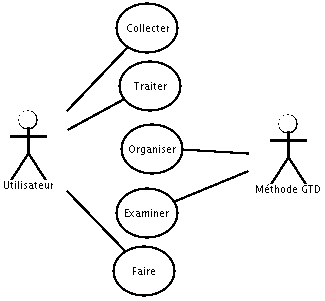
\includegraphics[width=7cm]{images/usecase.png}
\caption{Diagramme de cas d'utilisation}
\label{usecase}
\end{center}
\end{figure}

%%%%%%%%% USE CASE 1 %%%%%%%%%

\subsection{Collecter les informations}
L'objectif de ce cas d'utilisation est de recenser tout ce à quoi on pense et qu'on peut être amené à réaliser par la suite. Ces idées doivent pouvoir être notées rapidement, car elles peuvent apparaître à un moment où l'on est occupé (au téléphone, en réunion, etc.).

\subsubsection{Canevas de Cockburn}

\begin{usecase}{Collecter des choses à faire}
\begin{information}
\item[Goal in context~:] Récupérer des choses à faire et les ajouter à la liste de choses à faire
\item[Scope~:] La méthode GTD
\item[Level~:] Summary
\item[Pre-conditions~:] Avoir des choses à faire non classées dans GTD
\item[Post-conditions~:] Aucune chose à faire perdue
\item[Success End Condition~:] Toutes les choses à faire voulues ont été rentrées
\item[Failed End Condition~:] Les choses à faire données par l'utilisateur ont été perdues
\item[Primary actor~:] L'utilisateur, toute personne voulant être mieux organisée
\item[Trigger~:] L'utilisateur a demandé à rentrer des choses à faire
\\
\end{information}
\begin{scenario}
\item L'utilisateur demande à ajouter des choses à faire
\item La méthode GTD enregistre les choses à faire
\item L'utilisateur arrête la saisie
\\
\end{scenario}
\begin{relatedinformation}
\item[Priority~:] Faible
\item[Performance target~:] Quelques secondes par chose à faire
\item[Frequency~:] Régulièrement (potentiellement tous les jours)
\item[Channel to primary actor~:] Action directe de l'utilisateur
\\
\end{relatedinformation}
\begin{openissues}
\item Que se passe-t-il si le système perd une ou plusieurs choses à faire~?
\\
\end{openissues}
\end{usecase}

\subsubsection{Instantané}
Avant application de ce cas d'utilisation (figure \ref{collect1}), on obtient une liste des choses à faire auquelles on a ajouté des éléments (figure \ref{collect2}).

\begin{figure}[!ht]
\begin{center}
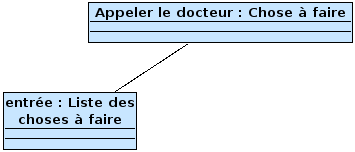
\includegraphics[width=6cm]{images/Instantane_Collect_1.png}
\caption{Etat du système \emph{avant} la collecte}
\label{collect1}
\end{center}
\end{figure}

\begin{figure}[!ht]
\begin{center}
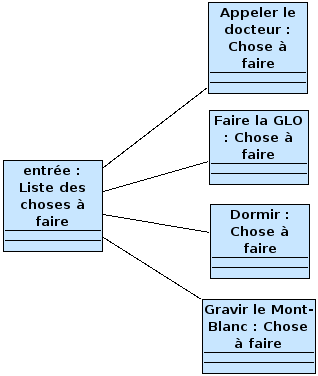
\includegraphics[width=6cm]{images/Instantane_Collect_2.png}
\caption{Etat du système \emph{après} la collecte}
\label{collect2}
\end{center}
\end{figure}

\subsubsection{Contraintes OCL}

Nous n'avons pas défini de contraintes OCL pour ce cas d'utilisation.

\subsubsection{Diagramme de séquence}
figure \ref{collectSequence}.
\begin{figure}[!ht]
\begin{center}
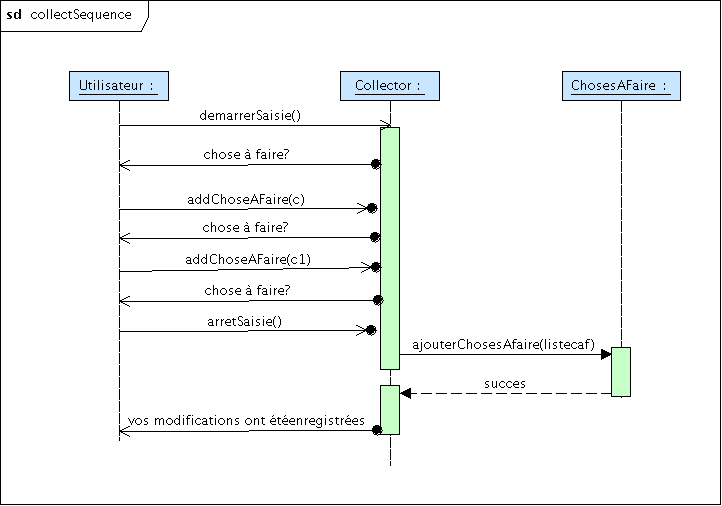
\includegraphics[width=12cm]{images/collectSequence.png}
\caption{Scénario de collecte des choses à faire}
\label{collectSequence}
\end{center}
\end{figure}


%%%%%%%%% USE CASE 2 %%%%%%%%%

\subsection{Traiter ces informations}
Après la collecte des informations, il faut leur appliquer un traitement afin connaître certaines propriétés essentielles pour le système, telles le contexte de la tâche, la périodicité, l'échéance, etc.

\subsubsection{Canevas de Cockburn}

\begin{usecase}{Collecter des choses à faire}
\begin{information}
\item[Goal in context~:] On effectue le traitement (création d'un projet contenant une décomposition de la tâche courante, ordonner à l'utilisateur de faire la tâche, la déléguer, la reporter, l'archiver) d'une ou plusieurs choses à faire de la liste
\item[Scope~:] La gestion des priorités après traitement, la création de la liste de choses à faire
\item[Level~:] Summary
\item[Pre-conditions~:] Liste de choses à faire non-vide
\item[Post-conditions~:] Les tâches traitées apparaissent dans les donnée stockée
\item[Success End Condition~:] Le chose à faire supprimée de la liste a été traitée
\item[Failed End Condition~:] Le traitement a échoué
\item[Primary actor~:] L'utilisateur
\item[Trigger~:] L'utilisateur
\\
\end{information}
\begin{scenario}
\item L'utilisateur demande à lancer le traitement des éléments de la liste des choses à faire
\item La méthode GTD émet une demande de renseignements des attributs de la chose à faire, en vue d'en faire une tâche
\item L'utilisateur rentre ou non des informations
\item La méthode GTD applique le traitement à la tâche ou le projet
\item La méthode GTD supprime la chose à faire qui vient d'être traitée
\item Arrêt de la procédure de traitement
\\
\end{scenario}
\begin{variation}
\item[3a] L'utilisateur rentre ou non des informations
\item[3a1] L'utilisateur effectue la tâche immédiatement et retour à l'étape 2.
\item[3a2] Il n'y a pas encore de contexte adapté à cette tâche, création d'un nouveau contexte.
\item[6a] L'utilisateur rentre ou non des informations et demande la chose à faire suivante
\item[6a1] On remplace l'arrêt du traitement par le retour à l'étape 2.
\\
\end{variation}
\begin{relatedinformation}
\item[Priority~:] Moyenne
\item[Performance target~:] Moins de deux minutes
\item[Frequency~:] Régulièrement (une fois par semaine)
\item[Channel to primary actor~:] Action directement effectuée par l'utilisateur
\\
\end{relatedinformation}
\begin{openissues}
\item Que se passe-t-il si la chose à faire n'est pas sauvegardée~?
\item Que se passe-t-il si la chose à faire n'est pas supprimée~?
\\
\end{openissues}
\end{usecase}

\subsubsection{Instantané}

Après traitement de données du système (figure \ref{process1}), des tâches sont créés et associées à des contextes (figure \ref{process2}).

\begin{figure}[!ht]
\begin{center}
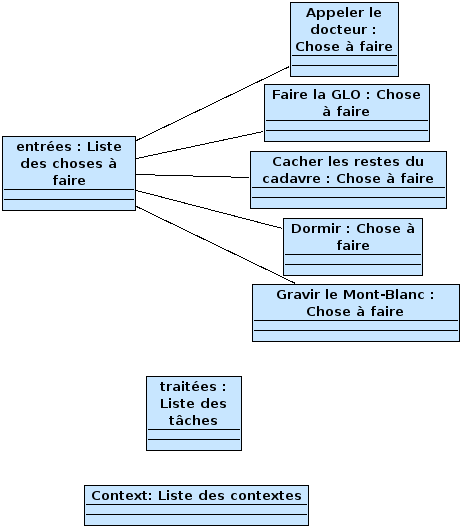
\includegraphics[width=10cm]{images/Instantane_Process_1.png}
\caption{Etat du système \emph{avant} le traitement}
\label{process1}
\end{center}
\end{figure}

\begin{figure}[!ht]
\begin{center}
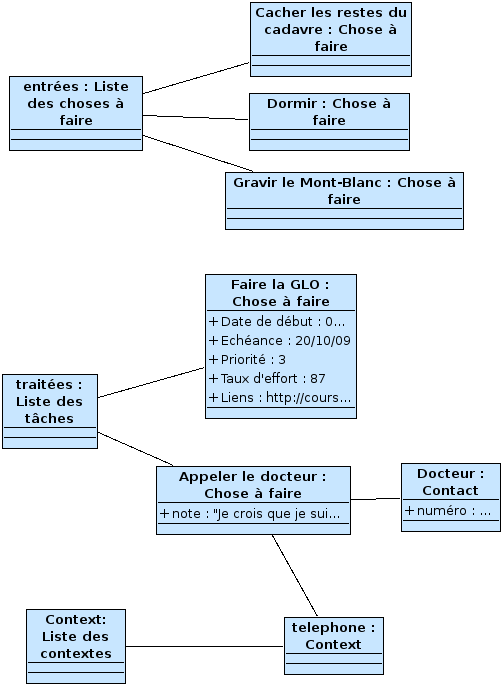
\includegraphics[width=10cm]{images/Instantane_Process_2.png}
\caption{Etat du système \emph{après} le traitement}
\label{process2}
\end{center}
\end{figure}

\subsubsection{Contraintes OCL}

\begin{ocl}
-- La taille de liste de choses a faire doit etre decrementee,
-- et au moins un conteneur de taches doit posseder des
-- elements supplementaires
context Traitement::traiterChoseAFaire()
pre Collector.getListeChoseAFaire().size() > 0
post Collector.getListeChoseAFaire().size()@pre >
		Collector.getListeChoseAFaire().size()
	and (NextAction.size() > NextAction.size()@pre
	or WaitFor.size() > WaitFor.size()@pre
	or Someday.size() > Someday.size()@pre
	or Archive.size() > Archive.size()@pre)
\end{ocl}

\subsubsection{Diagramme de séquence}
Dans le cas où la chose à faire correspond à une simple tâche, nous obtenons le diagramme de séquence de la figure \ref{traitementSequence}.
\begin{figure}[!ht]
\begin{center}
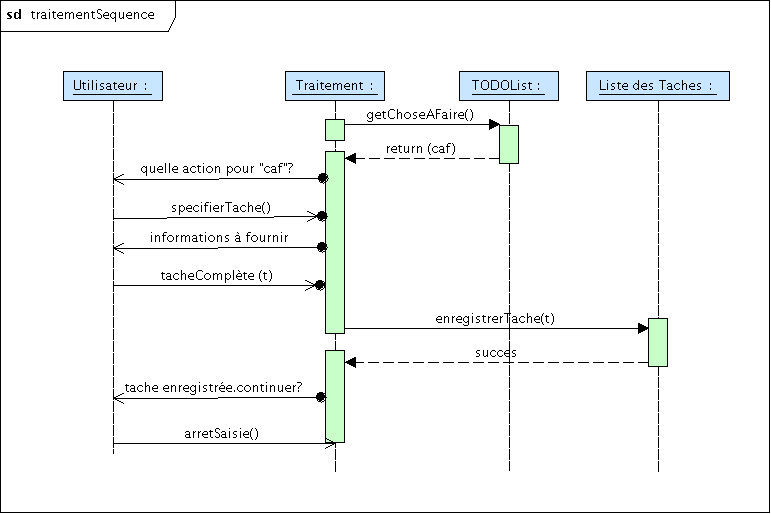
\includegraphics[width=12cm]{images/traitementSequence.png}
\caption{Scénario de traitement d'une chose à faire}
\label{traitementSequence}
\end{center}
\end{figure}

%%%%%%%%% USE CASE 3 %%%%%%%%%

\subsection{Organiser les tâches issues du traitement}

\subsubsection{Canevas de Cockburn}

\begin{usecase}{Organiser les éléments stockés dans les dossiers}
\begin{information}
\item[Goal in context~:] Gérer les priorités, les contextes et tout autres attributs pour définir l'ensemble des prochaines actions à partir des tâches dans les dossier.
\item[Scope~:] La création des tâches, leurs actions et leurs attributs.
\item[Level~:] Primary Task
\item[Pre-conditions~:] /
\item[Post-conditions~:] /
\item[Success End Condition~:] Toutes les tâches ont été triées.
\item[Failed End Condition~:] Tâches inorganisable, erreur système.
\item[Primary actor~:] Le système
\item[Trigger~:] Après le traitement/Après chaque modification
\\
\end{information}
\begin{scenario}
\item Le système requiert de l'ordre
\item Les éléments mal-placés ou entrants sont déplacés au bon endroit
\\
\end{scenario}
\begin{relatedinformation}
\item[Priority~:] Haute
\item[Performance target~:] Invisible à l'utilisateur
\item[Frequency~:] Après le traitement/Après chaque modification
\\
\end{relatedinformation}
\begin{openissues}
\item Que se passe-t-il dans le cas de conflit priorité/échéance ?
\\
\end{openissues}
\end{usecase}


\subsubsection{Instantané}

Avant organisation (figure \ref{organize1}), nous avons une liste de tâches dont les éléments se font spécifier (figure \ref{organize2}).

\begin{figure}[!ht]
\begin{center}
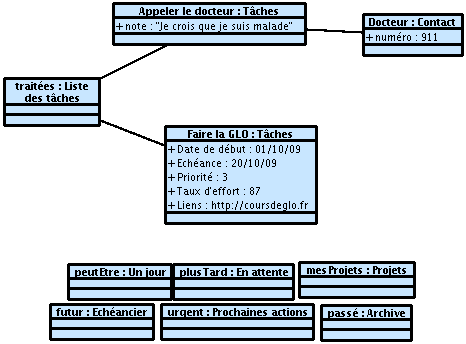
\includegraphics[width=10cm]{images/Instantane_Organize_1.png}
\caption{Etat du système \emph{avant} l'organisation}
\label{organize1}
\end{center}
\end{figure}

\begin{figure}[!ht]
\begin{center}
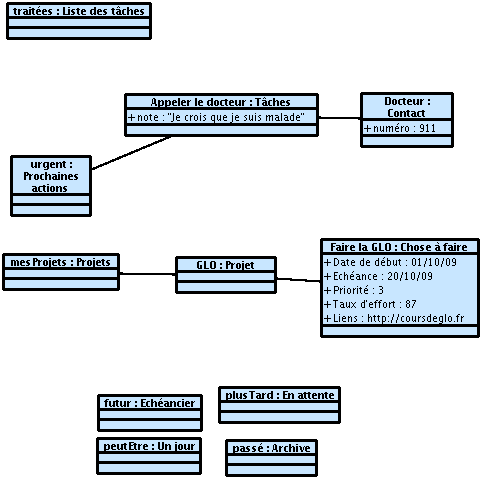
\includegraphics[width=10cm]{images/Instantane_Organize_2.png}
\caption{Etat du système \emph{après} l'organisation}
\label{organize2}
\end{center}
\end{figure}

\subsubsection{Contraintes OCL}

Nous n'avons pas défini de contraintes OCL pour ce cas d'utilisation.

\subsubsection{Diagramme de séquence}
Le scénario de l'organisation des tâches est décris par la figure \ref{organizeSequence}.
\begin{figure}[!ht]
\begin{center}
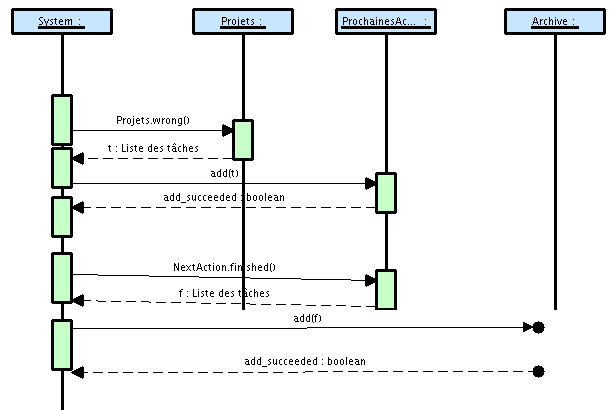
\includegraphics[width=12cm]{images/organizeSequence.png}
\caption{Scénario d'organisation des tâches}
\label{organizeSequence}
\end{center}
\end{figure}


%%%%%%%%% USE CASE 4 %%%%%%%%%

\subsection{Examiner régulièrement ces tâches et ajouter celles en attente}

\subsubsection{Canevas de Cockburn}

\begin{usecase}{Vérification des données stockées}
\begin{information}
\item[Goal in context~:] Vérifier si aucune tâche dans En Attente ou dans Un Jour n'est passée à l'état actif  et met l'échéancier à jour..
\item[Scope~:] Les tâches
\item[Level~:] Primary Task
\item[Pre-conditions~:] Il y a des tâches à examiner.
\item[Post-conditions~:] L'échéancier a été mis à jour.
\item[Success End Condition~:] Toutes les tâches examinées ont été activées
\item[Failed End Condition~:] Erreur système.
\item[Primary actor~:] Le système
\item[Trigger~:] Automatique
\\
\end{information}
\begin{scenario}
\item Vérifier dans En Attente si des tâches sont devenues actives
\item Vérifier dans Un Jour si il est possible de réaliser une tâche
\item Vérification si il y a un jour1 dans l'échéancier, et, si c'est le cas, ajoute ses projets dans le dossier Projets (en ajoutant sa première tâche dans Prochaines Actions) .
\item Mettre à jour l'échéancier
\item Transférer les tâches dans Prochaines Action
\\
\end{scenario}
\begin{relatedinformation}
\item[Priority~:] Haute
\item[Frequency~:] Une fois par jour
\\
\end{relatedinformation}
\end{usecase}

\subsubsection{Instantané}

Avant l'examen des tâches (figure \ref{review1}), nous avons une organisation qui va être remaniée par cette opération (figure \ref{review2}).

\begin{figure}[!ht]
\begin{center}
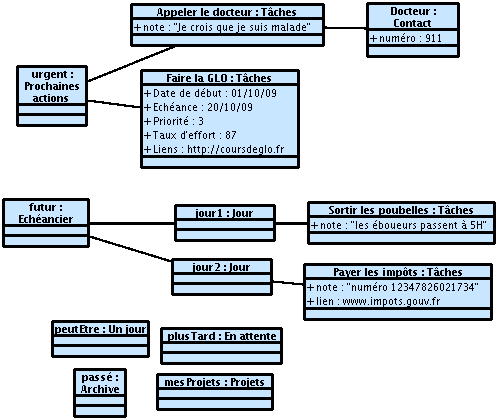
\includegraphics[width=10cm]{images/Instantane_Review_1.png}
\caption{Etat du système \emph{avant} la mise à jour des tâches de l'échéancier}
\label{review1}
\end{center}
\end{figure}

\begin{figure}[!ht]
\begin{center}
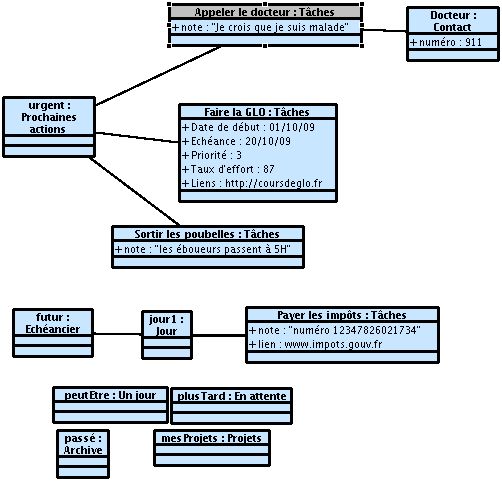
\includegraphics[width=10cm]{images/Instantane_Review_2.png}
\caption{Etat du système \emph{après} la mise à jour des tâches de l'échéancier}
\label{review2}
\end{center}
\end{figure}

\subsubsection{Contraintes OCL}

\begin{ocl}
-- Il doit au moins y avoir une tache a examiner
context Examen::review())
pre WaitFor.size() > 0
	or Someday.size() > 0
	or Echeancier.size() > 0
post Echeancier.jour1.getEcheance() = Date.today()
\end{ocl}

\subsubsection{Diagramme de séquence}
Le scénario type de ce cas d'utilisation est décris par la figure \ref{reviewSequence}.
\begin{figure}[!ht]
\begin{center}
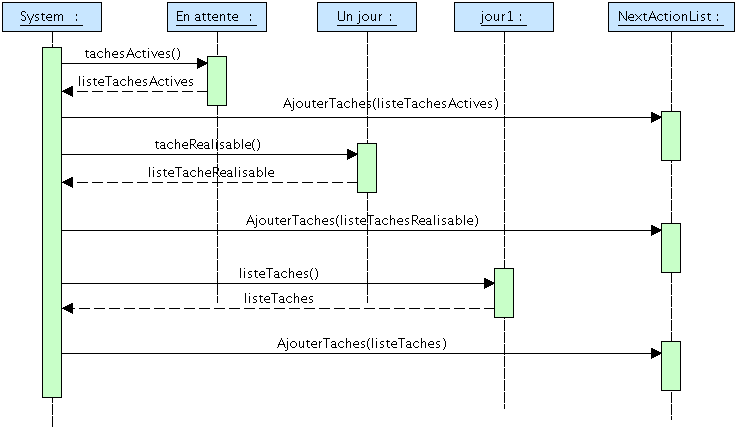
\includegraphics[width=12cm]{images/reviewSequence.png}
\caption{Scénario du cas d'utilisation examen}
\label{reviewSequence}
\end{center}
\end{figure}

%%%%%%%%% USE CASE 5 %%%%%%%%%

\subsection{Sélectionner une tâche afin de la réaliser}

\subsubsection{Canevas de Cockburn}

\begin{usecase}{Réaliser une tâche}
\begin{information}
\item[Goal in context~:] Obliger l'utilisateur à effectuer la tâche la plus prioritaire dans le dossier Prochaines Actions dans son contexte.
\item[Scope~:] Le contenu des Prochaines Actions
\item[Level~:] PrimaryTask
\item[Pre-conditions~:] L'utilisateur a du temps pour réaliser une tâche et il y a des tâches à effectuer.
\item[Post-conditions~:] L'utilisateur à réalisée la tâche prédéfini.
\item[Success End Condition~:] Ancienne tâche archivée et la seconde Prochaine Action devient la première.
\item[Failed End Condition~:] La tâche n'a pas été supprimée ou l'utilisateur n'a pas réalisé son travail.
\item[Primary actor~:] L'utilisateur
\item[Trigger~:] L'utilisateur
\\
\end{information}
\begin{scenario}
\item L'utilisateur demande à faire une tâche
\item L'utilisateur donne le contexte dans lequel il se trouve.
\item La méthode GTD choisit la tâche.
\item L'utilisateur indique qu'il a fini la tâche
\item La tâche est supprimée
\item Mise à jour des Prochaines Actions
\item L'utilisateur ne fait plus d'actions
\\
\end{scenario}
\begin{extension}
\item[4a] L'utilisateur n'a pas fini la tâche.
\item[4a1] La méthode GTD ne modifie rien.
\item[7a] L'utilisateur demande une nouvelle tâche à faire
\item[7a1] Retour à l'étape 3.
\\
\end{extension}
\begin{variation}
\item[6.1] Si une tâche est En Attente de la tâche réalisée, le système doit en informer l'utilisateur comme Prochaine Action à réaliser.
\\
\end{variation}
\begin{relatedinformation}
\item[Priority~:] Haute
\item[Frequency~:] Le plus souvent possible
\\
\end{relatedinformation}
\begin{openissues}
\item Que se passe-t-il si l'utilisateur ne finit jamais de tâches~?
\\
\end{openissues}
\end{usecase}

\subsubsection{Instantané}

Avant la réalisation de la tâche (figure \ref{do1}), la prochaine tâche devant être exécuté est (dans notre exemple) d'appeler un docteur. Cette tâche est alors désignée pour être terminée (figure \ref{do2}).

\begin{figure}[!ht]
\begin{center}
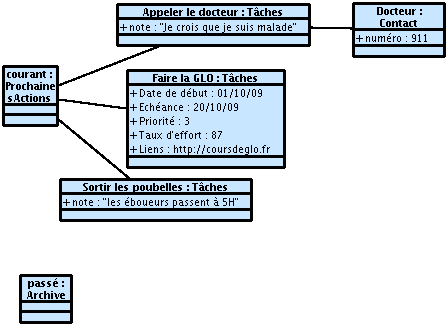
\includegraphics[width=10cm]{images/Instantane_Do_1.png}
\caption{Etat du système \emph{avant} la réalisation d'une tâche}
\label{do1}
\end{center}
\end{figure}

\begin{figure}[!ht]
\begin{center}
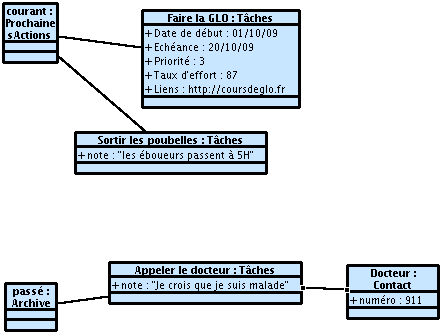
\includegraphics[width=10cm]{images/Instantane_Do_2.png}
\caption{Etat du système \emph{après} la réalisation d'une tâche}
\label{do2}
\end{center}
\end{figure}

\subsubsection{Contraintes OCL}

\begin{ocl}
-- Une fois la tache "NextAction" accomplie, celle qui etait
-- en deuxieme sur la liste des actions devient la
-- nouvelle "NextAction"
context Do::do()
pre NextAction.size() > 0
post NextAction.second()@pre = NextAction.first()
\end{ocl}

\subsubsection{Diagramme de séquence}
Le scénario de la réalisation d'une tâche est décrit par la figure \ref{doSequence}.
\begin{figure}[!ht]
\begin{center}
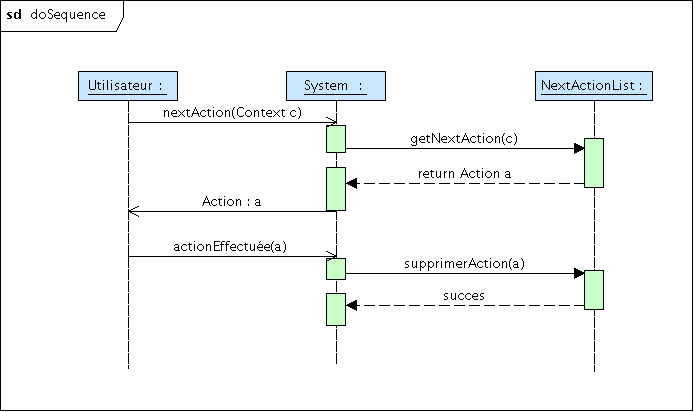
\includegraphics[width=12cm]{images/doSequence.png}
\caption{Scénario de réalisation d'une tâche}
\label{doSequence}
\end{center}
\end{figure}

\chapter{Analyse finale}

L'analyse de tous les cas d'utilisation du système nous a permis de concevoir le diagramme de classe de la figure \ref{ddc}.

\begin{figure}[!ht]
\begin{center}
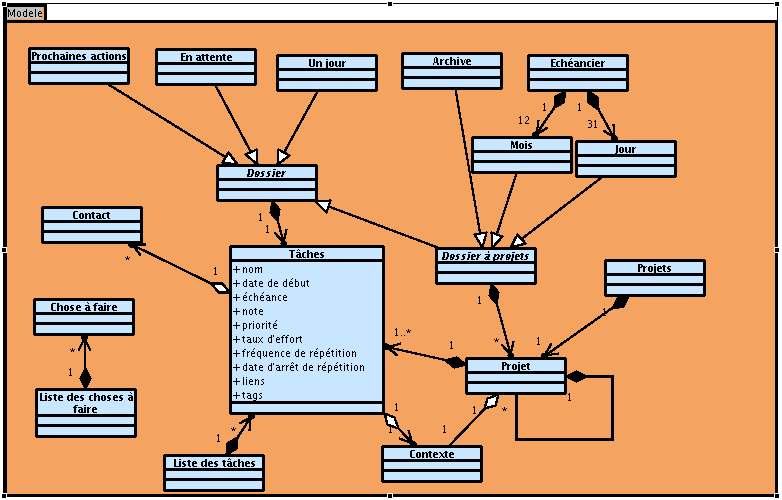
\includegraphics[width=12cm]{images/DiagrammedeClasse.png}
\caption{Diagramme de classes du modèle}
\label{ddc}
\end{center}
\end{figure}

\newpage
\section{Conclusion}

La modélisation du la méthode GTD nous a fait prendre conscience de certains aspects du problème auxquels nous n'avions pas pensé, et nous a fait réaliser à quel point chaque membre du groupe avait une vision foncièrement différente de la solution.
En effet, il s'est avéré que nous n'étions pratiquement jamais en accord sur chaque cas d'utilisation, et il nous a fallu creuser le problème beaucoup plus en profondeur pour savoir qui avait l'idée la meilleure.
Une fois toutes les notions clairement définies, l'avancement du projet a accéléré car nous pouvions alors travailler en équipe de manière beaucoup plus rigoureuse et efficace.



\chapter{Spécification d'exigences logicielles}

\setcounter{minitocdepth}{1}
\minitoc

% Template proposé par "The Unified Process for EDUcation (UPEDU)"
% http://www.yoopeedoo.org/upedu/

%Selon le wikipedia \url{http://fr.wikipedia.org/wiki/Exigence_(ingénierie)}
%De bonnes exigences doivent être :
% * Nécessaires – Elles doivent porter sur des éléments nécessaires, c'est-à-dire des éléments importants du système que d'autres composants du système ne pourraient pas compenser.
% * Non ambiguës – Elles doivent être susceptibles de n'avoir qu'une seule interprétation.
% * Concises – Elles doivent être énoncées dans un langage qui soit précis, bref et agréable à lire, et qui de plus communique l'essence de ce qui est exigé.
% * Cohérentes – Elles ne doivent pas contredire d'autres exigences établies, ni être contredites par d'autres exigences. De plus, elle doit, d'un énoncé d'exigence au suivant, utiliser des termes et un langage qui signifie la même chose.
% * Complètes – Elles doivent être énoncées entièrement en un endroit et d'une façon qui ne force pas le lecteur à regarder un texte supplémentaire pour savoir ce que l'exigence signifie.
% * Accessibles – Elles doivent être réalistes quant à aux moyens mis en œuvre en termes d'argent disponible, avec les ressources disponibles, dans le temps disponible.
% * Vérifiables – Elles doivent permettre de déterminer si elles ont été atteintes ou non selon l'une de quatre méthodes possibles : inspection, analyse, démonstration, ou test.

\section{Introduction}
%L’introduction donne une vue d’ensemble de tout le document. On y présente toute information que le lecteur a besoin pour  comprendre le document. Elle comprend l’objectif du document, sa portée, les définitions, acronymes et abréviations, les références et une vue d’ensemble du document.
%Note : La SEL comporte l’ensemble des exigences logicielles pour une portion ou pour tout le système. La présente spécification est adaptée pour  un projet utilisant une modélisation de cas d’utilisation. Cet artéfact est un paquetage qui comprend les cas d’utilisation du modèle des cas d’utilisation et les spécifications supplémentaires applicables ainsi que les autres informations pertinentes.
%Plusieurs aménagements d’une SEL sont possibles. La norme (IEEE830-1998) est la référence pour de plus amples explications ainsi que pour d’autres options d’organisation du document.

Dans ce chapitre, nous allons spécifier les fonctionnalités du logiciel per\-met\-tant de mettre en pratique la méthode GTD pour un particulier.
 On utilisera donc l'analyse effectuée dans le chapitre précédent, en prenant en compte le fait que nous spécifions cette fois un logiciel, et non une méthode généraliste.


	\subsection{Objectif}
%Préciser les objectifs de ce chapitre. La SEL doit décrire le comportement externe de l’application ou du sous-système identifié. Elle décrit 	aussi les exigences non-fonctionnelles et les autres facteurs nécessaires à une description complète et compréhensible des exigences pour le logiciel.

L'objectif poursuivi est donc de décrire de manière précise le comportement et les fonctionnalités du futur logiciel GTD.
 Nous allons également lister toutes les conditions qu'il doit vérifier, ainsi que tous les facteurs extérieurs desquels il dépend.

	\subsection{Conventions}
%<Describe any standards or typographical conventions that were followed when writing this SRS, such as fonts or highlighting that have special significance. For example, state whether priorities  for higher-level requirements are assumed to be inherited by detailed requirements, or whether every requirement statement is to have its own priority.>


Nous assumerons dans ce documents que l'utilisateur est capable d'utiliser un ordinateur et est au courant des exigences et effets liés à cette utilisation.

	\subsection{Audience}
%<Describe the different types of reader that the document is intended for, such as developers, project managers, marketing staff, users, testers, and documentation writers. Describe what the rest of this SRS contains and how it is organized. Suggest a sequence for reading the document, beginning with the overview sections and proceeding through the sections that are most pertinent to each reader type.>

Ce document est essentiellement destiné aux développeurs du projet et au chef de projet, car ce sont eux qui devront mettre en place ce qui y est décrit.
Cependant, le responsable de la relation client devra vérifier que c'est bien ce qui est attendu, et les testeurs devront s'y référer.
Accessoirement, il doit être compréhensible, et apprécié par le correcteur.

	\subsection{Portée du document}
%Une brève description de la portée de ce document, l’application qu’il décrit, les caractéristiques ou autres sous-systèmes auxquels l’application est associée, le ou les modèles de cas d’utilisation qu’il décrit ainsi que tout autre chose qui peut être influencée ou affectée par ce document.

Nous décrivons ici une application client instrumentant la méthode GTD, destinée à un usage professionnel et/ou personnel. L'application visée a pour but d'être accessible pour un assez large public, mais pourra éventuellement dépendre (dans le cas d'une utilisation professionnelle en particulier) d'un serveur distant.
On devra donc également prendre en compte cette dépendance dans les spécifications.
On décrira dans les parties suivantes des cas d'utilisation représentatifs des principales fonctionnalités offertes par le logiciel.

	\subsection{Définitions, acronymes et abréviations}
	%Énumérer les définitions de tous les termes, acronymes et abréviations nécessaires à la compréhension du document d’architecture logicielle. Cette information peut renvoyer à l’artéfact Glossaire du projet..

	Voir Dictionnaire de données (partie 1).


	%\subsection{Références}
%Cette section comporte la liste de tous les documents cités dans le document. Chaque document doit être identifié par son titre, son numéro, lorsque applicable, sa date et l’organisation qui l’a publiée. Les sources qui peuvent fournir les références doivent être citées. Cette dernière information peut être elle-même une référence à une annexe ou à un autre document.



	%\subsection{Organisation du chapitre}
%Cette section décrit le contenu du reste du document  et explique comment le document est organisé.

\section{Description générale}
%<Décrire les principaux facteurs qui affectent le produit et ses exigences. On n’y énonce pas des exigences spécifiques, mais on y fournit une toile de fond aux exigences qui sont définies en détail à la section 3 afin d’en faciliter la compréhension. Cela comprend les items suivants:>

Le logiciel que nous concevons devra respecter un certain nombre de spé\-ci\-fi\-ca\-tions provenant de différentes sources~: utilisateur, système d'exploitation ou encore la méthode GTD. Ces spécifications concernent un large éventail d'aspects du logiciel~:


	\subsection{Perspectives du produit}
%<Describe the context and origin of the product being specified in this SRS. For example, state whether this product is a follow-on member of a product family, a replacement for certain existing systems, or a new, self-contained product. If the SRS defines a component of a larger system, relate the requirements of the larger system to the functionality of this software and identify interfaces between the two. A simple diagram that shows the major components of the overall system, subsystem interconnections, and external interfaces can be helpful.>

Le logiciel que nous développons s'inscrit dans la suite de logiciel de style GTD.
Nous développons plus particulièrement le composant représentant la partie logiciel client d'un système client/serveur.
\\
Le produit final fera l'interface entre un utilisateur et son compte GTD stocké sur le serveur. Le logiciel sera capable d'accéder aux informations du serveur (réception/envoi), mais aussi de fonctionner hors connexion (de faire la mise à jour sur le serveur plus tard ou de permettre une utilisation complètement locale).

\begin{figure}
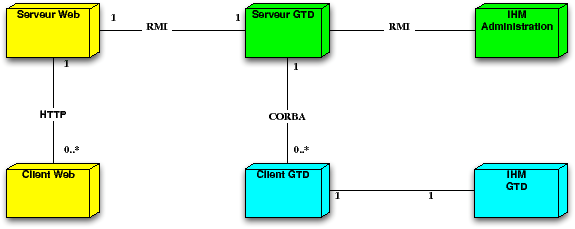
\includegraphics[width=12cm]{images/projet-gtd001}
\end{figure}


	\subsection{Fonctions du produit}
%<Décrire brièvement les fonctions principales du logiciel. Par exemple : >
%<Les fonctions d’un système de gestion peuvent être la maintenance d’un compte client, accéder à l’état de compte du client et produire la facturation.>
Le logiciel comportera différents sous-systèmes offrant chacun plusieurs fonctionnalités.
Un système de gestion des ``choses à faire/idées''~: enregistrements de nouvelles idées à partir de l'utilisateur, demande à l'utilisateur des informations sur chaque idées pour appliquer un traitement.
\\
Un système de gestion des tâches : place les tâches dans les catégories adéquates, vérifie si les tâches en attente doivent le rester, supprimer/archiver les tâches achevées.
Il devra également disposer des éléments suivants :
\begin{itemize}
\item Un système de connexion utilisateur : connexion , déconnexion, préférences (changement du mot de passe, ...).
\item Un système connexion au serveur : envoi (immédiat ou différé), réception (globale ou par paquets).
\item Un système de cryptage/décryptage.
\end{itemize}



	\subsection{Caractéristiques et classes d'utilisateurs}
%<Décrire les caractéristiques générales des utilisateurs qui ont un impact sur les exigences du document. Cela inclut le niveau de scolarité, l’expérience et l’expertise technique.>
%<Identify the various user classes that you anticipate will use this product. User classes may be differentiated based on frequency of use, subset of product functions used, technical expertise, security or privilege levels, educational level, or experience. Describe the pertinent characteristics of each user class. Certain requirements may pertain only to certain user classes. Distinguish the favored user classes from those who are less important to satisfy.>

Nous comptons orienter notre logiciel pour cibler les utilisateurs ayant de nombreuses choses à faire et qui ont besoin de s'organiser.
\\
Le client pourra être aussi bien un homme d'affaire qu'un artisan, la seule nécessité est que le client ait un réel besoin d'organisation.
\\
Nous projetons de développer le logiciel pour qu'un utilisateur lambda puisse l'utiliser. Un minimum de connaissance sera nécessaire mais pas plus que pour la méthode GTD elle-même.
\\
Ce sont souvent les personnes occupées qui ont le plus besoin d'organisation, ces personnes utiliseront probablement le logiciel tous les jours car ils auront besoin  d'ajouter ou de réaliser des tâches souvent.

	\subsection{Environnement opérationnel}
%<Describe the environment in which the software will operate, including the hardware platform, operating system and versions, and any other software components or applications with which it must peacefully coexist.>

Nous prévoyons que notre logiciel puisse être exécuter sur différents systèmes d'exploitation (MacOS, Linux, Windows). Il sera nécessaire que ce système d'exploitation possède une machine virtuelle Java.
\\
Pour l'utilisation avec un serveur, une connexion (réseau ou internet) sera nécessaire pour la liaison avec lui.

	\subsection{Contraintes de conception et d'implémentation}
%<Describe any items or issues that will limit the options available to the developers. These might include: corporate or regulatory policies; hardware limitations (timing requirements, memory requirements); interfaces to other applications; specific technologies, tools, and databases to be used; parallel operations; language requirements; communications protocols; security considerations; design conventions or programming standards (for example, if the customer’s organization will be responsible for maintaining the delivered software).>

Dans le but de déployer notre logiciel sur un grand nombre de plateformes, nous avons décidé de le développer en Java.
\\
Pour une harmonie et un code propre, nous développerons un checkstyle\footnote{outil de contrôle de code, permet de vérifier le style d'un code source} pour notre projet.


	\subsection{Documentation utilisateur}
%<List the user documentation components (such as user manuals, on-line help, and tutorials) that will be delivered along with the software. Identify any known user documentation delivery formats or standards.>

Nous comptons écrire trois types de documentation:

\begin{itemize}
\item une aide en ligne (dans le logiciel) en html~;
\item un manuel (fichier texte décrivant les principales manipulations) en pdf~;
\item un tutoriel vidéo sur YouTube\footnote{\url{http://www.youtube.com/}}.
\end{itemize}


	\subsection{Hypothèses et dépendances}
%<Décrire tout élément de faisabilité technique, disponibilité de sous-système ou de composant ou toute autre hypothèse liée au projet de laquelle dépend la viabilité du logiciel.>
%<List any assumed factors (as opposed to known facts) that could affect the requirements stated in the SRS. These could include third-party or commercial components that you plan to use, issues around the development or operating environment, or constraints. The project could be affected if these assumptions are incorrect, are not shared, or change. Also identify any dependencies the project has on external factors, such as software components that you intend to reuse from another project, unless they are already documented elsewhere (for example, in the vision and scope document or the project plan).>

On assume que le mode de connexion et le format des données pour communiquer avec le serveur sont normalisés avec l'équipe de développement du serveur GTD.


\subsection{Exigences reportées}
%<Énumérer les exigences qui peuvent être réalisées dans des versions futures du système.>

Etant soumis à des contraintes temporelles, nous avons choisi de reporter la spécification des intégrations avec des logiciels déjà présents sur la machine (calendrier, liste de contacts, etc.).



\section{Fonctionnalités du logiciel}
%Décrire les exigences fonctionnelles du système qui peuvent être exprimées et langage naturel.
%Pour plusieurs applications, c’est la partie principale de la SEL et son organisation doit, par conséquent, être bien réfléchie.
%Elle est habituellement hiérarchisée par caractéristiques, mais elle peut l’être par uti\-li\-sa\-teur ou par sous-système.
%Les exigences fonctionnelles peuvent inclure les caractéristiques, les capacités et la sécurité.

%Lorsque des outils de développement, tels des référentiels d’exigences ou des outils de modélisation, sont utilisés, on peut référer à ces données en indiquant l’endroit et le nom de cet outil.

Dans cette section, nous reprenons les cas d'utilisation de la méthode GTD et nous les adaptons pour un système informatique.
	\subsection{Collecte des choses à faire}

Le logiciel permet de recenser les choses à faire, de manière rapide et simple, à n'importe quel moment (y compris pendant l'exécution d'une autre tâche par le logiciel).


	\subsubsection{Description}
% Utilisez le canevas de cockburn pour décrire le cas d'utilisation
% Indiquez la priotité: Haute, Moyenne et Basse
% Indiquez, éventuellement, des mesures spécifiques, comme le profit, le coût, les risques, etc.
% (sur une échelle relative d'un minimum de 1 à un maximum de 9))

	\begin{usecase}{Collecter des choses à faire}
	\begin{information}
	\item[Goal in context~:] Récupérer des choses à faire et les ajouter à la liste de choses à faire
	\item[Scope~:] La méthode GTD
	\item[Level~:] Summary
	\item[Pre-conditions~:] L'utilisateur est identifié, et a des choses à faire non classées dans le système
	\item[Post-conditions~:] Toutes les choses à faire sont enregistrées.
	\item[Success End Condition~:] Toutes les choses à faire désirées ont été enregistrées pour l'utilisateur.
	\item[Failed End Condition~:] Les choses à faire données par l'utilisateur ont été perdues
	\item[Primary actor~:] L'utilisateur, toute personne voulant être mieux organisée
	\item[Trigger~:] L'utilisateur a demandé à rentrer des choses à faire
	\\
	\end{information}
	\begin{scenario}
	\item L'utilisateur demande à ajouter des choses à faire
	\item Le système enregistre les choses à faire tant que l'utilisateur en ajoute
	\item L'utilisateur arrête la saisie
	\\
	\end{scenario}
	\begin{relatedinformation}
	\item[Priority~:] Moyenne
	\item[Performance target~:] Quelques secondes par chose à faire
	\item[Frequency~:] Régulièrement (potentiellement tous les jours, ou même plusieurs fois par jour)
	\item[Channel to primary actor~:] Action directe de l'utilisateur
	\\
	\end{relatedinformation}
	\begin{openissues}
	\item Que se passe-t-il si le système perd une ou plusieurs choses à faire?
	\\
	\end{openissues}
	\end{usecase}



	\subsubsection{Exigences fonctionnelles}
%<Itemize the detailed functional requirements associated with this feature. These are the software capabilities that must be present in order for the user to carry out the services provided by the feature, or to execute the use case. Include how the product should respond to anticipated error conditions or invalid inputs. Requirements should be concise, complete, unambiguous, verifiable, and necessary. Use “TBD” as a placeholder to indicate when necessary information is not yet available.>

%<Each requirement should be uniquely identified with a sequence number or a meaningful tag of some kind.>

%REQ-1:
%REQ-2:
\begin{description}
 \item[EXIGE-1~:] L'ajout de nouvelle chose à faire doit être disponible à tout moment, quel que soit la tâche effectuée par le système.
 \item[EXIGE-2~:] Dès qu'une chose à faire est ajoutée, elle est sauvegardée de manière persistante, même si la saisie ne s'arrête pas.
 \end{description}






	\subsection{Traitement}

	Le logiciel permet de passer en revue les choses à faire une à une, et offre la possibilité à l'utilisateur de choisir le traitement  à effectuer : le faire tout de suite (implique suppression de la chose à faire), transformation en tâche (et spécification de la tâche), transformation en projet (et spécification de la première tâche de ce projet au moins) ou en sous-projet.


\subsubsection{Description}

	\begin{usecase}{Traitement}
	\begin{information}
	\item[Goal in context~:] On effectue le traitement (création d'un projet contenant une décomposition de la tâche courante, l'utilisateur effectue la tâche, la délègue, la reporte, l'archive) d'une ou plusieurs choses à faire de la liste
	\item[Scope~:] La gestion des priorités après traitement, la création de la liste de choses à faire
	\item[Level~:] Summary
	\item[Pre-conditions~:] Liste de choses à faire non-vide
	\item[Post-conditions~:] Les tâches traitées apparaissent dans les donnée stockée
	\item[Success End Condition~:] Le chose à faire supprimée de la liste a été traitée (et la tâche a été effectuée, déléguée, transformée, ...)
	\item[Failed End Condition~:] Le traitement a échoué
	\item[Primary actor~:] L'utilisateur
	\item[Trigger~:] L'utilisateur
	\\
	\end{information}
	\begin{scenario}
	\item L'utilisateur demande à lancer le traitement des choses à faire.
	\item Le système lui affiche la première chose à faire
	\item Le système demande le traitement adéquat à appliquer (voir Goal)
	\item L'utilisateur entre des informations, afin de créer la tâche ou le projet correspondant à la chose à faire
	\item Le système enregistre la tâche ou le projet
	\item Le système supprime la chose à faire qui vient d'être traitée
	\item Arrêt de la procédure de traitement
	\\
	\end{scenario}

	\begin{variation}
	\item[4a.] L'utilisateur entre des informations, afin de créer la tâche ou le projet correspondant à la chose à faire
	\item[4a1.] L'utilisateur effectue la tâche immédiatement, et saut à l'étape 6.
	\item[4a2.] Il n'y a pas encore de contexte adapté à cette tâche, création d'un nouveau contexte.
	\item[7a.] Arrêt de la procédure de traitement
	\item[7a1.] On remplace l'arrêt du traitement par le retour à l'étape 2 (on passe à la chose à faire suivante).
	\\
	\end{variation}

	\begin{relatedinformation}
	\item[Priority~:] Moyenne
	\item[Performance target~:] Moins de deux minutes par chose à faire
	\item[Frequency~:] Régulièrement (une fois par semaine?)
	\item[Channel to primary actor~:] Action directement effectuée par l'utilisateur
	\\
	\end{relatedinformation}
	\begin{openissues}
	\item Que se passe-t-il si la tâche créée n'est pas sauvegardée~?
	\item Que se passe-t-il si la chose à faire n'est pas supprimée~?
	\\
	\end{openissues}
	\end{usecase}


\subsubsection{Exigences fonctionnelles}

\begin{description}
\item[EXIGE-3~:] Le traitement doit pouvoir être interrompu à tout moment, et on doit pouvoir le reprendre à l'endroit exact ou l'on était rendu.
\item[EXIGE-4~:] Une tâche ou un projet créé lors du traitement doit immédiatement être sauvegardé de manière persistante.
\item[EXIGE-5~:] Une fois qu'une chose à faire a été traitée, elle doit être supprimée de la liste.
\item[EXIGE-6~:] Lors d'une création (de tâche ou de projet), tous les champs obligatoire doivent être renseigné, afin de permettre l'organisation automatique des tâches.
 \end{description}


	\subsection{Organisation}

\subsubsection{Description}

\begin{usecase}{Organiser les éléments stockés dans les dossiers}
\begin{information}
\item[Goal in context~:] Gérer les priorités, les contextes et tout autres attributs pour définir l'ensemble des prochaines actions à partir des tâches existantes.
\item[Scope~:] La création des tâches, leurs actions et leurs attributs.
\item[Level~:] Primary Task
\item[Pre-conditions~:] avoir des tâches déjà créées.
\item[Post-conditions~:]
\item[Success End Condition~:] Toutes les tâches ont été triées.
\item[Failed End Condition~:] Tâches inorganisable, signalisation à l'utilisateur.
\item[Primary actor~:] Le système
\item[Trigger~:] Après le traitement/Après chaque modification
\\
\end{information}
\begin{scenario}
\item Le système étudie une à une les tâches existantes et calcule leur priorité
\item Le système trie toutes les tâches en fonction de leur priorité (la plus forte priorité en tête)
\\
\end{scenario}
\begin{variation}
\item[2a.] Deux tâches ont exactement la même priorité
\item[2a1.] Le système indique au sein de la tâche qu'il place avant l'autre qu'il existe également une autre tâche de même priorité~; l'utilisateur sera en conséquent averti en temps voulu
\end{variation}
\begin{relatedinformation}
\item[Priority~:] Haute
\item[Performance target~:] Invisible à l'utilisateur
\item[Frequency~:] Après le traitement/Après chaque modification
\\
\end{relatedinformation}
\begin{openissues}
\item Que se passe-t-il dans le cas de conflit priorité/échéance ?
\\
\end{openissues}
\end{usecase}


\subsubsection{Exigences fonctionnelles}
\begin{description}
 \item[EXIGE-7~:] L'organisation des taches doit pouvoir se faire sans intervention humaine
 \end{description}



	\subsection{Revue}

Le logiciel passe régulièrement en revue toutes les tâches, afin de redéfinir les priorités de chacune (par exemple, dans le cas ou une tâche arrive très bientôt à sa date d'échéance).

\subsubsection{Description}

\begin{usecase}{Vérification des données stockées}
\begin{information}
\item[Goal in context~:] Vérifier si aucune tâche dans En Attente ou dans Un Jour n'est passée à l'état actif  et met l'échéancier à jour.
\item[Scope~:] Les tâches
\item[Level~:] Primary Task
\item[Pre-conditions~:] Il y a des tâches à examiner.
\item[Post-conditions~:] L'échéancier a été mis à jour.
\item[Success End Condition~:] Toutes les tâches examinées ont été activées
\item[Failed End Condition~:] Erreur système.
\item[Primary actor~:] Le logiciel
\item[Trigger~:] Au démarrage de l'application ou à minuit
\\
\end{information}
\begin{scenario}
\item Vérifier dans En Attente si des tâches sont devenues actives
\item Vérifier dans Un Jour si il est possible de réaliser une tâche
%\item Vérification si il y a un jour1 dans l'échéancier, et, si c'est le cas, ajoute ses projets dans le dossier Projets (en ajoutant sa première tâche dans Prochaines Actions) .
\item Mettre à jour l'échéancier
\item Transférer les tâches dans Prochaines Action
\\
\end{scenario}
\begin{relatedinformation}
\item[Priority~:] Haute
\item[Frequency~:] A chaque fois qu'un utilisateur démarre le logiciel ou au moins une fois par jour
\\
\end{relatedinformation}
\end{usecase}

\subsubsection{Exigences fonctionnelles}

\begin{description}
 \item[EXIGE-8~:] Le passage en revue doit pouvoir être interrompu rapidement et à tout moment, et on doit pouvoir le reprendre à l'endroit exact ou l'on était rendu.
 \end{description}

	\subsection{Faire}

Le logiciel renvoie, en fonction d'un contexte donné par l'utilisateur, la (ou les) tâche(s) prioritaire(s).

\subsubsection{Description}

\begin{usecase}{Réaliser une tâche}
\begin{information}
\item[Goal in context~:] Proposer à l'utilisateur d'effectuer la tâche la plus prioritaire du dossier Prochaines Actions, dans le contexte ou il se trouve.
\item[Scope~:] Le contenu des Prochaines Actions
\item[Level~:] PrimaryTask
\item[Pre-conditions~:] L'utilisateur a du temps pour réaliser une tâche et il y a des tâches à effectuer.
\item[Post-conditions~:] L'utilisateur à réalisée la tâche prédéfini.
\item[Success End Condition~:] Ancienne tâche archivée et la seconde Prochaine Action devient la première.
\item[Failed End Condition~:] La tâche n'a pas été supprimée ou l'utilisateur n'a pas réalisé son travail.
\item[Primary actor~:] L'utilisateur
\item[Trigger~:] L'utilisateur
\\
\end{information}
\begin{scenario}
\item L'utilisateur demande à faire une tâche
\item L'utilisateur donne le contexte dans lequel il se trouve.
\item Le logiciel choisit la tâche.
\item L'utilisateur indique qu'il a fini la tâche
\item La tâche est supprimée
\item Mise à jour des Prochaines Actions
\item L'utilisateur ne fait plus d'actions
\\
\end{scenario}
\begin{extension}
\item[4a.] L'utilisateur n'a pas fini la tâche.
\item[4a1.] Le logiciel ne modifie rien.
\item[7a.] L'utilisateur demande une nouvelle tâche à faire
\item[7a1.] Retour à l'étape 3.
\\
\end{extension}
\begin{variation}
\item[6.1.] Si une tâche est En Attente de la tâche réalisée, le système doit recalculer sa priorité, éventuellement la placer comme Prochaine Action à réaliser.
\\
\end{variation}
\begin{relatedinformation}
\item[Priority~:] Haute
\item[Frequency~:] A chaque fois que l'utilisateur demande une tâche à effectuer
\\
\end{relatedinformation}
\begin{openissues}
\item Que se passe-t-il si l'utilisateur ne finit jamais de tâches~?
\\
\end{openissues}
\end{usecase}

\subsubsection{Exigences fonctionnelles}

\begin{description}
 \item[EXIGE-9~:] Quand il demande une tâche à faire, l'utilisateur doit toujours récupérer la même tâche pour un contexte donné tant qu'elle n'est pas finie.%pour pas le perturber et douter du choix imposé
 \item[EXIGE-10~:] Quand il demande une tâche à faire, l'utilisateur doit tout de même pouvoir sélectionner une tâche différente de celle proposée si il estime qu'elle ne convient pas.
 \end{description}

%%%%%%%%% USE CASE 6 %%%%%%%%%

\subsection{Authentification de l'utilisateur}

\subsubsection{Canevas de Cockburn}

\begin{usecase}{Authentification d'un utilisateur sur le logiciel}
\begin{information}
\item[Goal in context~:] Authentifier un utilisateur pour qu'il ait accès à ces données cryptées
\item[Scope~:] Le logiciel
\item[Level~:] Primary Task
\item[Pre-conditions~:] L'utilisateur est enregistré
\item[Post-conditions~:] L'utilisateur est authentifié
\item[Success End Condition~:] L'utilisateur est authentifié
\item[Failed End Condition~:] L'utilisateur n'est pas authentifié
\item[Primary actor~:] L'utilisateur
\item[Trigger~:] L'utilisateur
\\
\end{information}
\begin{scenario}
\item L'utilisateur demande à s'authentifier
\item Le logiciel lui affiche une fenêtre d'authentification
\item L'utilisateur rentre ses identifiants
\item Le système vérifie si les identifiants sont corrects
\item L'utilisateur est authentifié
\\
\end{scenario}

\begin{extension}
\item[4a.] Les identifiants sont incorrects
\item[4a1.] Retour à l'étape 2
\\
\end{extension}

\begin{variation}
\item[3.1.] L'utilisateur a oublié son mot de passe; le logiciel le lui renvoie par e-mail.
\\
\end{variation}

\begin{relatedinformation}
\item[Priority~:] Haute
\item[Performance target~:] Obligatoire
\item[Frequency~:] A chaque lancement du logiciel
\\
\end{relatedinformation}

\end{usecase}

\subsubsection{Diagramme d'activité}
L'authentification de l'utilisateur est représenté par le diagramme d'activité \ref{authentActivite}.
\begin{figure}[!ht]
\begin{center}
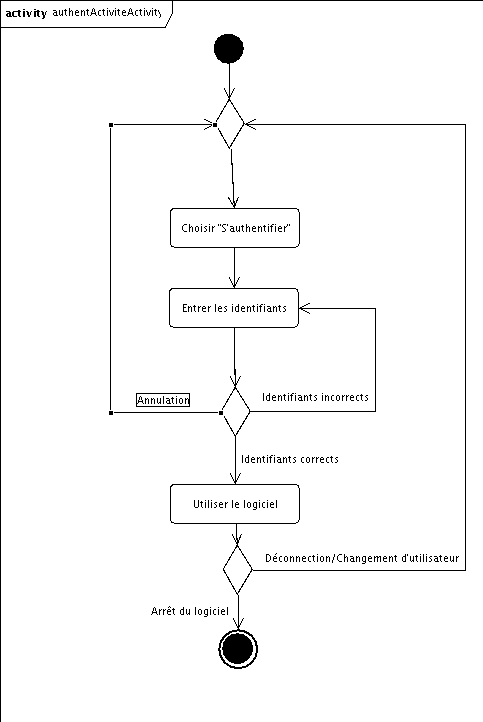
\includegraphics[width=12cm]{images/authentActivite.png}
\caption{Diagramme d'activité de l'authentification de l'utilisateur}
\label{authentActivite}
\end{center}
\end{figure}


%%%%%%%%% USE CASE 7 %%%%%%%%%

\subsection{Connection au serveur}

\subsubsection{Canevas de Cockburn}

\begin{usecase}{Synchroniser les données avec le serveur}
\begin{information}
\item[Goal in context~:] Se connecter avec le serveur pour mettre à jour les données
\item[Scope~:] Le serveur
\item[Level~:] Summary
\item[Pre-conditions~:] disposer d'une interface réseau active
\item[Post-conditions~:] déconnexion du serveur réussie
\item[Success End Condition~:] les données ont été synchronisé
\item[Failed End Condition~:] la synchronisation a échouée
\item[Primary actor~:] Le logiciel
\item[Trigger~:] Fréquence déterminée dans les préférences utilisateur/ Déclenchement manuel de l'utilisateur
\\
\end{information}
\begin{scenario}
\item Le logiciel envoi des données modifiées au serveur
\item Le serveur retourne les données qui ont été modifiées sur lui et pas sur le client
\\
\end{scenario}

\begin{extension}
\item[2a.] Des conflits de mises à jour apparaissent : on a besoin de l'utilisateur pour les gérer
\\
\end{extension}

\begin{variation}
\item[1.1.] La connexion avec le serveur est perdue; une synchronisation ultérieure est programmée.
\item[1.2.] Le serveur demande une authentification; le logiciel doit s'authentifier auprès du serveur.
\\
\end{variation}

\begin{relatedinformation}
\item[Priority~:] Faible
\item[Performance target~:] Invisible à l'utilisateur
\item[Frequency~:] Fréquence déterminée dans les préférences utilisateur/ Déclenchement manuel de l'utilisateur
\\
\end{relatedinformation}
\begin{openissues}
\item Que se passe-t-il dans le cas de conflit de date entre les données en ligne et locales ?
\\
\end{openissues}
\end{usecase}


\subsubsection{Diagramme d'activités}
L'échange avec le serveur est décrit par le diagramme d'activités \ref{connectionActivite}.
\begin{figure}[!ht]
\begin{center}
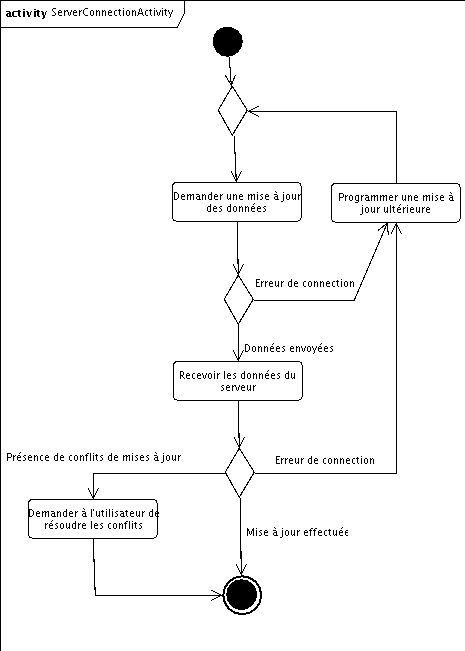
\includegraphics[width=12cm]{images/connectionActivite.png}
\caption{Diagramme d'activité de la synchronisation avec le serveur}
\label{connectionActivite}
\end{center}
\end{figure}


\section{Exigences des interfaces externes}
	\subsection{Interface utilisateur}
%<Describe the logical characteristics of each interface between the software product and the users. This may include sample screen images, any GUI standards or product family style guides that are to be followed, screen layout constraints, standard buttons and functions (e.g., help) that will appear on every screen, keyboard shortcuts, error message display standards, and so on. Define the software components for which a user interface is needed. Details of the user interface design should be documented in a separate user interface specification.>

\subsubsection{IHM}
L'IHM\footnote{Interface Homme Machine} doit être claire et non ambigüe.
Elle doit disposer d'un bouton très accessible "Nouvelle chose à faire" ainsi que de "Traitement des choses à faire".
Les tâches doivent être triées par contexte et accessibles de manière intuitive (onglets ou arborescence).
Elle doit disposer d'un accès aisé à la prochaine action et aux informations la composant.

Si nous devions créer une première interface, notre premier jet pourrais ressembler au logiciel Getting Things Gnome\cite{gettingThingsGnome}. (voir illustration \ref{gettingThingsGnome})

\begin{figure}[!ht]
\begin{center}
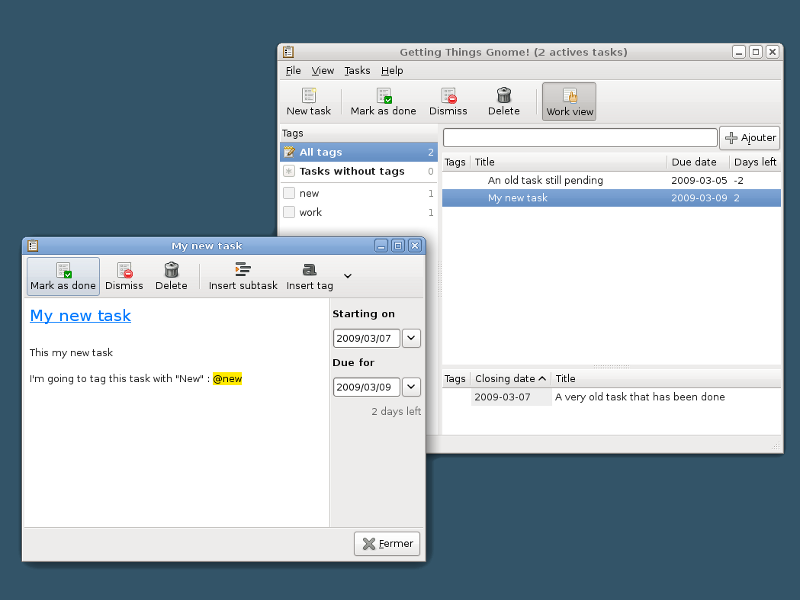
\includegraphics[width=12cm]{images/gettingThingsGnome.png}
\caption{Screenshot du logiciel Getting Things Gnome}
\label{gettingThingsGnome}
\end{center}
\end{figure}

Lors des prochains livrables, nous devons organiser l'IHM selon le canevas de présentation vu dans le cours du même nom.

\subsubsection{Aides contextuelles}
L'interface doit disposer d'aides contextuelle sur tous les éléments de menus et icônes, et d'éventuellement une aide en ligne.
De plus, on peut ajouter des informations qui dépendent de l'expérience de l'utilisateur.

\subsubsection{Documentation}
Elle doit comprendre, de manière distincte :
\begin{itemize}
 \item explications simples et concises de la méthode GTD.
 \item explications rapides des fonctionnalités de base de l'outil.
 \item explications complètes de toutes les fonctionnalités de l'outil.
\end{itemize}

\subsubsection{Support de formation}
L'utilisateur doit pouvoir apprendre par lui-même à utiliser l'outil, à l'aide d'un tutoriel concis.

	\subsection{Interface matérielle}
%<Describe the logical and physical characteristics of each interface between the software product and the hardware components of the system. This may include the supported device types, the nature of the data and control interactions between the software and the hardware, and communication protocols to be used.>

La machine hôte doit disposer d'une connexion à internet, afin de pouvoir se connecter à un serveur distant.
Le programme devra être installé sur un ordinateur, car elle ne sera pas défini pour un appareil mobile.

	\subsection{Interface logicielle}
%<Describe the connections between this product and other specific software components (name and version), including databases, operating systems, tools, libraries, and integrated commercial components. Identify the data items or messages coming into the system and going out and describe the purpose of each. Describe the services needed and the nature of communications. Refer to documents that describe detailed application programming interface protocols. Identify data that will be shared across software components. If the data sharing mechanism must be implemented in a specific way (for example, use of a global data area in a multitasking operating system), specify this as an implementation constraint.>

La machine hôte devra disposer d'un système d'exploitation pouvant supporter l'environnement d'exécution Java\footnote{Le JRE actuel est la version 1.6} car Java est le langage de programmation le plus portable, et permettant un développement très rapide.
Nous ne savons pas encore quelles sont les bibliothèques ou bases de données qui seront utilisées. Ce point devra être éclairci lors des prochains livrables, voire lors de l'implémentation.

	\subsection{Interfaces ou protocoles de communication}
%<Describe the requirements associated with any communications functions required by this product, including e-mail, web browser, network server communications protocols, electronic forms, and so on. Define any pertinent message formatting. Identify any communication standards that will be used, such as FTP or HTTP. Specify any communication security or encryption issues, data transfer rates, and synchronization mechanisms.>

Le programme doit offrir la possibilité de se connecter au serveur par l'utilisation de CORBA.
L'interface de communication des objets doit nous être fournie par le serveur, et le programme doit pouvoir l'utiliser.
Nous devrons donc nous mettre d'accord avec l'équipe chargée de l'implémentation de cette interface.
Ce serveur pourra se trouver n'importe où, que ce soit sur une machine locale où sur internet.
La communication doit se faire de manière sécurisée (cryptée) et acquittée, de manière à ne pas avoir de doublons ou de pertes d'information.

	\subsection{Contraintes de mémoire}

Nous ne pouvons pas pour l'instant prédire combien de mémoire le programme utilisera~; nous compléterons ce point lors des prochains livrables.
Cependant, il parait évident que notre logiciel devant pouvoir être utilisé par un maximum de personnes, il devra pouvoir s'exécuter sur une machine disposant de ressources mémoire moyennes, voire basses (par rapport à la moyenne des ordinateurs particuliers).
Cela permettra également une réactivité accrue.

	%\subsection{Hypothèses et dépendances}

\section{Autres exigences non-fonctionnelles}

	\subsection{Utilisabilité}

	\subsubsection{Outil simple}
L'outil doit être aisément accessible à un utilisateur ne connaissant pas la méthode GTD~; cet utilisateur ne doit pas avoir à passer beaucoup de temps à se former sur l'outil avant d'être productif.

	\subsubsection{Outil complet}
L'outil doit répondre aux attentes d'un utilisateur expérimenté à la fois sur la méthode GTD et sur l'utilisation de cet outil, c'est à dire qu'il doit être en mesure d'effectuer toutes les opérations qu'il désire, notamment celles qui sont récurrentes, de manière très rapide et efficace.

	\subsubsection{Outil respectant les standards}
L'interface homme-machine doit respecter les standards des principaux développeurs de logiciels (Microsoft, Apple, etc.), afin d'être plus ergonomique et d'accélérer le processus d'adaptation de l'utilisateur à l'outil.


	\subsection{Fiabilité}

	\subsubsection{Disponibilité de l'outil}
L'outil nécessite de pouvoir fonctionner continuellement durant la période éveillée de son utilisateur, à cause de la saisie de choses à faire qui peut avoir lieu à n'importe quel moment.

	\subsubsection{Autres exigences de fiabilité}
A ce niveau d'avancement du projet, les autres exigences de fiabilité de l'outil ne peuvent pas encore être spécifiées, à savoir ~:
\begin{itemize}
 \item Durée moyenne de fonctionnement avant défaillance
 \item Durée moyenne de rétablissement
 \item Précision de l'outil
 \item Nombre maximum d'anomalies
 \item Criticité
\end{itemize}

	\subsection{Exigences de performance}
Nous ne pouvons pas encore définir ce type d'exigences au niveau actuel d'avancement du projet.


	\subsection{Maintenabilité}

	\subsubsection{Norme de codage}
Afin de faciliter la relecture de notre code, nous avons choisi de respecter des critères de codage que nous définirons dans notre checkstyle.


	\subsection{Exigences de sûreté}

	\subsubsection{Précautions à prendre}
Cet outil présente les mêmes risques que n'importe quel autre logiciel, notamment vis-à-vis de l'épilepsie ou de la fatigue visuelle due à l'écran.

	\subsubsection{Sûreté vis-à-vis de la perte de données}
Certaines données importantes de l'utilisateur n'existent qu'au sein de son outil~; il est donc primordial que ces données ne puissent pas être perdues.
De même, en cas d'erreur du programme ou du système, les données doivent être récupérées.


	\subsection{Exigences de sécurité}

	\subsubsection{Confidentialité des données}
Afin de préserver la confidentialité des données, chaque compte d'utilisateur doit être protégé par mot de passe.
Les fichiers assurant la persistance des données de l'utilisateur doivent également être sécurisé, par exemple à l'aide d'un cryptage.
De même, les données transitant sur Internet (notamment pour la mise à jour entre le client et le serveur) doivent elles aussi être cryptées.


	\subsection{Attribut de qualité logicielle}

%<Specify any additional quality characteristics for the product that will be important to either the customers or the developers. Some to consider are: adaptability, availability, correctness, flexibility, interoperability, maintainability, portability, reliability, reusability, robustness, testability, and usability. Write these to be specific, quantitative, and verifiable when possible. At the least, clarify the relative preferences for various attributes, such as ease of use over ease of learning.>

Le logiciel, de par le fait qu'il doit être adressé à un assez large public, devra présenter une grande facilité d'apprentissage.
Il devra néanmoins permettre, pour un utilisateur expérimenté, une utilisation fluide et efficace des fonctionnalités plus avancées.
En outre, L'application devra bien sûr être la plus réactive possible (moins de deux secondes pour une action) pour offrir une utilisation agréable, et être assez robuste pour des systèmes (matériel et OS) peu efficaces.

\section{Autres exigences}
%<Define any other requirements not covered elsewhere in the SRS. This might include database requirements, internationalization requirements, legal requirements, reuse objectives for the project, and so on. Add any new sections that are pertinent to the project.>

Nous ne pouvons pour l'instant définir les autre exigences du logiciel qui sera développé. Ce points sera à éclaircir lors des prochains livrables.

\section{Classification des exigences fonctionnelles}

%Énumérer dans un tableau toutes les exigences fonctionnelles et leur type, essentielle, souhaitable ou optionnelle.
%Elles peuvent être triées par leur ordre d’apparition dans le document ou par type.

\begin{center}
\begin{tabular}{|p{1.7cm}|p{8cm}|p{1.7cm}|}
\hline
Code & Exigence & Type\\
\hline
EXIGE-1 & L'ajout de nouvelle chose à faire doit être disponible à tout moment, quel que soit la tâche effectuée par le système. & essentielle\\
\hline
EXIGE-2 & Dès qu'une chose à faire est ajoutée, elle est sauvegardée de manière persistante, même si la saisie ne s'arrête pas. & essentielle\\
\hline
EXIGE-3 & Le traitement doit pouvoir être interrompu à tout moment, et on doit pouvoir le reprendre à l'endroit exact ou l'on était rendu. & souhaitable\\
\hline
EXIGE-4 & Une tâche ou un projet créé lors du traitement doit immédiatement être sauvegardé de manière persistante. & essentielle\\
\hline
EXIGE-5 & Une fois qu'une chose à faire a été traitée, elle doit être supprimée de la liste. & essentielle\\
\hline
EXIGE-6 & Lors d'une création (de tâche ou de projet), tous les champs obligatoire doivent être renseigné, afin de permettre l'organisation automatique des tâches. & essentielle\\
\hline
EXIGE-7 & L'organisation des taches doit pouvoir se faire sans intervention humaine & souhaitable\\
\hline
EXIGE-8 & Le passage en revue doit pouvoir être interrompu rapidement et à tout moment, et on doit pouvoir le reprendre à l'endroit exact ou l'on était rendu. & souhaitable\\
\hline
EXIGE-9 & Quand il demande une tâche à faire, l'utilisateur doit toujours récupérer la même tâche pour un contexte donné tant qu'elle n'est pas finie. & souhaitable\\
\hline
EXIGE-10 & Quand il demande une tâche à faire, l'utilisateur doit tout de même pouvoir sélectionner une tâche différente de celle proposée si il estime qu'elle ne convient pas. & essentielle\\
\hline
\end{tabular}
\end{center}


\section{Conclusion}

Maintenant que nous avons définis tous nos critères et toutes nos exigences, nous pouvons nous concentrer sur finir l'analyse pour pouvoir enfin réaliser notre logiciel.


\chapter{Spécification des composants}

\minitoc

\section{Introduction}

	\subsection{Objectif}
Notre architecture étant conséquente, nous devons déterminer les différents composants du système et leur assemblage, afin d'en avoir une meilleur perception.
Notre point de vue se situe à un haut niveau, afin de décrire les exigences de chaque composant.
Il ne s'agit pas pour l'instant de savoir comment sera constitué chacun des composants.

	\subsection{Organisation du chapitre}
%Cette section décrit le contenu du reste du chapitre  et explique comment le document est organisé.
Dans un premier temps, nous essaierons de présenter chacun des composants principaux du système.
Nous aborderons ensuite les différentes interactions entre les composants par le biais de cas d'utilisation.
Nous devrons enfin spécifier les interfaces des différents composants, et spécifier les types d'objets qu'il nous sera nécessaire de créer.

\section{Description des composants}

%Établir les frontières du système.
Une des partie les plus délicates est de définir les frontières entre les différents concepts.

Nous avons choisi de définir un composant ControleCentral qui régit l'ensemble du programme.
Ce composant sera chargé d'utiliser les services fournis par d'autres composants internes.
Nous appellerons ces différents composants: Authentification, Gestionnaire de persistance et MethodeGTD.
Ces trois composants forment une base de l'application, qui devra néanmoins être étoffée pour obtenir un système complètement fonctionnel.
Un composant doit nous permettre la communication avec le serveur. Nous le nommerons donc CommunicationServeur.
Nous aurons également besoin d'un autre composant qui sera chargé du cryptage des données et du hachage du mot de passe, que ce soit en local sur la machine, ou pour la communication avec le serveur distant\footnote{si le serveur nous permet d'utiliser ce genre de fonctionnalités}.

Voyons maintenant cela plus en détail.

%Division du système en composants.

L'agencement des différents composants est décrit dans le schéma ci-dessous : 

\begin{figure}[htbp]
	\centering
		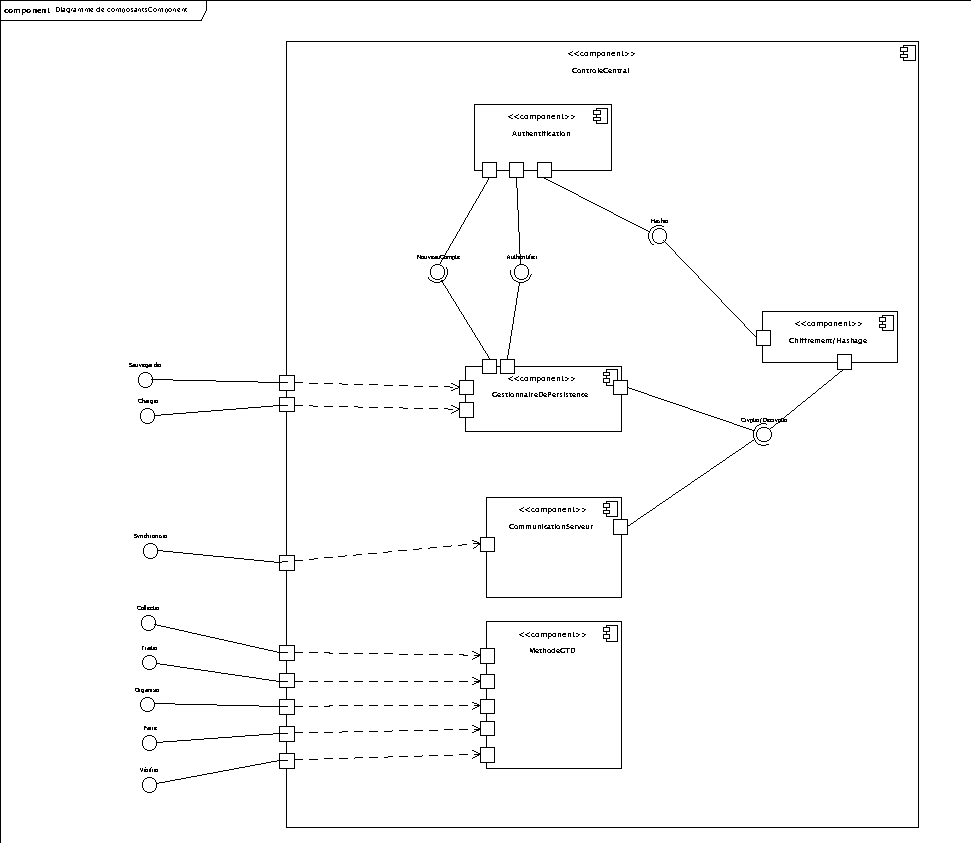
\includegraphics[width=15cm]{images/L3/composants.png}
	\caption{Le composant ControleCentral et ses interfaces}
	\label{fig:ControleCentral}
\end{figure}

%Décrire le comportement souhaité des composants.

\subsection{Le composant ControleCentral}

Voici le composant ControleCentral et les interfaces des services qu'il fourni.
C'est par lui que devront transiter toutes les méthodes.
Cela permettra de garder une gestion cohérente du système. %, en évitant à un futur développeur de créer un controleur .
Nous avons choisi de représenter ce composant global car il nous paraissait évident de le faire figurer, mais nous ne pouvions pas en faire un composant extérieur aux autres car il ne fourni aucune interface, il se contente d'organiser ses composants interne.
Il s'agit donc plus d'une configuration qu'un composant, car il contient tous les autres composants du système.

\subsection{Le composant MethodeGTD}

C'est le composant principal du système.
Il permet d'effectuer les différentes opérations de la méthode GTD sur la structure de donnée.

\subsection{Le composant Chiffrement/Hachage}

Ce composant aura deux tâches bien distinctes : 

\begin{enumerate}
\item il permettra le chiffrement des données pour la sauvegarde des fichiers en local, ainsi que pour la communication avec le serveur.
\item il permettra également le hachage des mots de passe, afin que ceux-ci ne puissent être dévoilés.
\end{enumerate}


\subsection{Le composant Authentification}

%Comme son nom l'indique, ce composant permettra l'authentification des différents utilisateurs du système.
Cet outil devant pouvoir être utilisé potentiellement par plusieurs utilisateurs, le système aura besoin d'un composant capable de gérer les authentifications de chacun d'eux.
Il doit donc permettre d'indiquer si un mot de passe donné est bien celui correspondant au login de l'utilisateur.

\subsection{Le composant GestionnaireDePersistence}

Le système devant pouvoir être utilisé uniquement de manière locale, nous devons pouvoir gérer la persistance des données, de manière à ce que l'utilisateur puisse éteindre son ordinateur par exemple.
Nous devrons alors enregistrer notre structure de donnée sous forme de fichier.
Ce composant aura aussi la responsabilité de charger les données d'un utilisateur contenues dans la base, après avoir vérifié son login et mot de passe.

\subsection{Le composant CommunicationServeur}

Ce composant a été défini afin de pouvoir communiquer avec le serveur.
Il devra permettre la synchronisation des données entre le client local et le serveur distant, par le biais d'une communication cryptée.
La représentation des données n'étant pas forcément identique entre le client et le serveur, le composant devra donc effectuer un travail de conversion des données.




\section{Interactions}

Dans ce qui suit, nous allons décrire les interactions principales entre les principaux acteurs de notre système.
On se focalisera en particulier sur les cas d'utilisation qui seront le plus souvent rencontrés.

%Décrire, à haut-niveau, la collaboration entre les composants majeurs, en faisant référence aux besoins.
Voici, à haut niveau, la manière dont les différents composants collaborent entre eux.
// 
Toutes les actions sont initiées par le composant ControleCentral( avec lequel interagira l'utilisateur). Les opérations complexes sur le compte actif sont effectuées par le composant MethodeGTD, mais la persistance des modifications est lancée par ControleCentral, et effectuée par le gestionnaire de persistance.
Le chargement d'un compte utilisateur est effectuée par le gestionnaire de persistance. Celui-ci utilise le composant Authentification, pour savoir quel compte charger, et le composant Chiffrement, pour décrypter les données stockées.//
L'authentification utilise également le composant Chiffrement(ou du moins sa fonction de hachage), afin de comparer le login et le mot de passe entrés avec ceux existants.
Enfin, le composant CommunicationServeur utilise également le Chiffrement pour crypter la communication distante.



%Utiliser des interactions, c'est à dire, des diagrammes de séquence et des diagrammes de communication. Utiliser éventuellement des diagrammes d'activités.

%\emph{Ne vous limitez pas à une seule interaction par cas d'utilisation}

\subsection{Traiter une chose a faire }

\begin{figure}[!htbp]
\centering
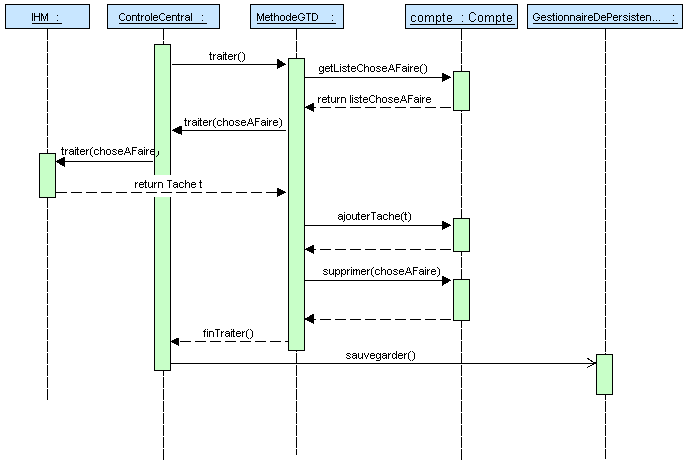
\includegraphics[width=12cm]{images/L3/diagrammeSequence/Traiter.png}
\caption{Interaction \--- Traiter \-- Création d'une tâche}
\label{traiterSequence}
\end{figure}

Dans le premier diagramme \ref{traiterSequence}  , on peut voir la séquence d'appel intervenant lors du traitement d'une Chose A Faire, lorsque celle-ci donne lieu à la création d'une tâche.
\\
Dans le diagramme suivant \ref{traiterActivite}, on peut voir les différents chemins que peut prendre l'algorithme de traitement. On peut y voir les possibilités de création de projet, sous-projet, projet ordonné(dépendance entre les tâches) etc.


\begin{figure}[!htbp]
\centering
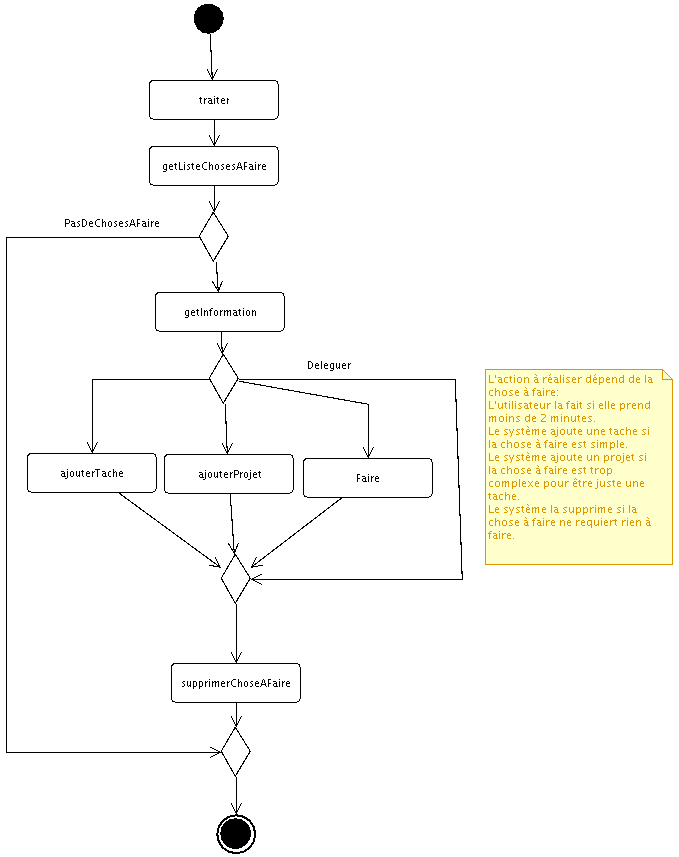
\includegraphics[width=12cm]{images/L3/diagrammeActivite/Traiter.png}
\caption{Interaction \--- Traiter \-- vue générale}
\label{traiterActivite}
\end{figure}

\subsection{Organiser des tâches}

Dans le diagramme \ref{organizeSequence}, on peut observer une séquence du cas Organiser. 

\begin{figure}[!htbp]
\centering
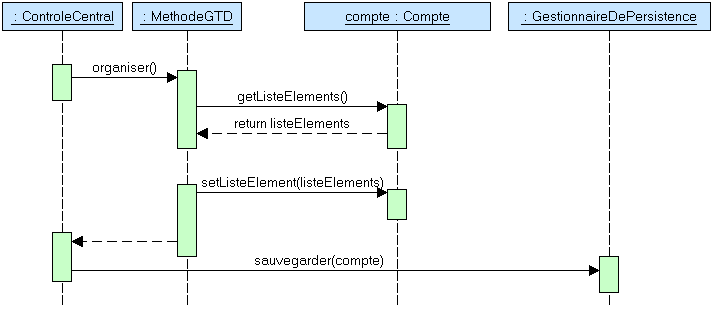
\includegraphics[width=12cm]{images/L3/diagrammeSequence/organiser.png}
\caption{Interaction \--- Organiser}
\label{organizeSequence}
\end{figure}

\subsection{Examen des tâches}

Le diagramme \ref{examinerSequence} représente l'examen des tâches.

\begin{figure}[!htbp]
\centering
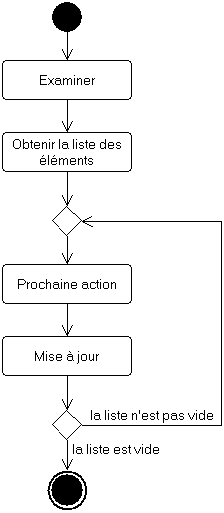
\includegraphics[scale=0.5]{images/L3/diagrammeActivite/examiner.png}
\caption{Interaction \--- Examiner}
\label{examinerSequence}
\end{figure}

\subsection{Faire une tâche}

Le diagramme \ref{doSequence} représente l'action de faire une tâche.

\begin{figure}[!htbp]
\centering
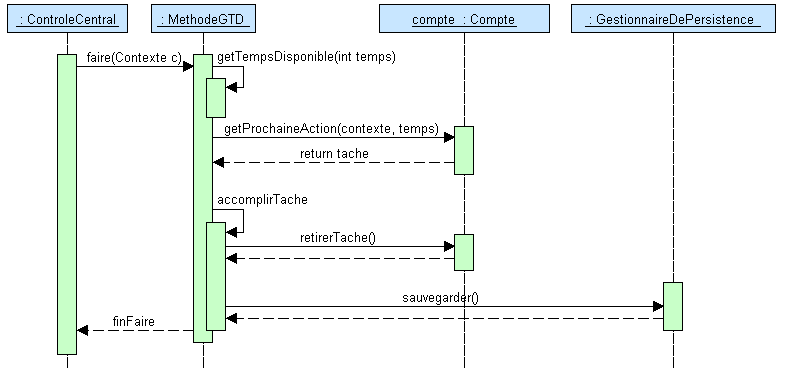
\includegraphics[width=12cm]{images/L3/diagrammeSequence/faire.png}
\caption{Interaction \--- Faire}
\label{doSequence}
\end{figure}

\subsection{Authentification d'un utilisateur}

Le diagramme d'activité \ref{authSequence} représente l'authentification des utilisateurs.

\begin{figure}[!htbp]
\centering
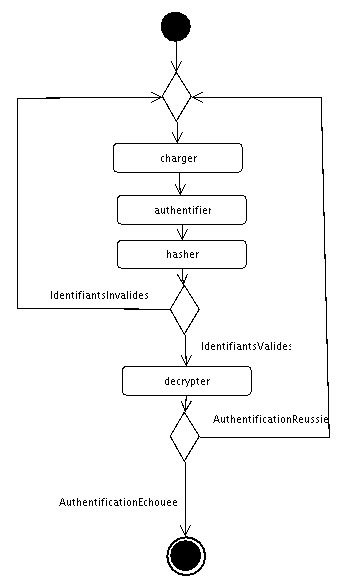
\includegraphics[width=12cm]{images/L3/diagrammeActivite/authentification.png}
%faudrai en faire un...
\caption{Interaction \--- Authentifier}
\label{authSequence}
\end{figure}

\section{Spécification des interfaces}

	\subsection{Interface du composant MethodeGTD}

		\begin{itemize}
			\item \code{collecter(idee : String) : void} \\
			Permet de collecter un nouvelle idée
			\begin{ocl}
-- L'idee doit exister
context collecter(idee : String) : void
pre: idee <> null
	and idee.size()>0
			\end{ocl}

			\item \code{traiter(idee : ChoseAFaire) : Tache} \\
			Renseigne une idée, pour la transformer en tâche.

			\item \code{organiser() : void} \\
			Calcule la priorité dynamique des tâches, et les ordonne selon cette priorité.

			\item \code{verifier(listeTache : Tache[*]) : void} \\
			Passe en revue une liste de tâches, pour mettre à jour la priorité dynamique.

			\item \code{faire(listeTache : Tache[*], contexte : Contexte) : Tache} \\
			Sélectionne la tâche la plus importante à faire selon un contexte donné.
		\end{itemize}

	\subsection{Interface du composant GestionnaireDePersistance}

	L'interface du gestionnaire de persistance autorise le chargement/enregistrement d'un compte à partir/depuis un fichier à l'aide d'un login et d'un mot de passe.

		\begin{itemize}
			\item \code{sauvegarder() : void} \\
			Permet de sauvegarder le compte lié au login de l'utilisateur
			\item \code{charger(login : String, motDePasse : String) : Comptes} \\
			Charge et renvoie le compte lié au login si le mot de passe est correct.
			\item \code{enregistrerIdentifiants(tableCleValeur : Map<String, String>) : void} \\
			Enregistre la table des identifiants et mots de passe cryptés dans un fichier.
			\item \code{chargerIdentifiants() : Map<String, String>} \\
			Charge la table des identifiants et mots de passe cryptés depuis un fichier.
		\end{itemize}

Nous avons définit la fonction sauvegarder comme ceci car le gestionnaire de persistance gardera en mémoire l'identifiant du compte chargé, ou bien pourra le récupérer depuis le contrôle central, qui devra être un singleton.
Nous verrons la meilleure façon de faire lors de l'implémentation.

	\subsection{Interface du composant Chiffrement/Hachage}

	L'interface du ce composant permet le chiffrement et le déchiffrement de fichier ainsi que le hachage (pour des mots de passe typiquement).

		\begin{itemize}
			\item \code{crypter(entree : Fichier) : Fichier} \\
			Crypte un fichier donné dans un autre fichier.
			\item \code{decrypter(entree : Fichier) : Fichier} \\
			Décrypte un fichier donné et restitue un fichier non crypté.
			\item \code{hasher(motDePasse : String) : String} \\
			Crypte le mot de passe de manière unidirectionnel.
		\end{itemize}

Concernant le cryptage/décryptage, nous nous sommes basés sur des fichiers pour l'instant, bien que nous ne sachons pas comment ce système pourra être représenté.
Il pourrait s'agir de transformer un Compte en chaine de caractères cryptée.
Nous verrons cela plus en détail lors de l'implémentation.

	\subsection{Interface du composant Authentification}

	L'interface de ce composant permet l'authentification des utilisateur.

		\begin{itemize}
			\item \code{authentifier(nom : String, motDePasse : String) : boolean} \\
			Authentifie ou non un utilisateur suivant un mot de passe donné.
			\item \code{nouveauCompte(nom : String, motDePasse : String) : void} \\
			Associe un nouvel utilisateur et son mot de passe.
			\begin{ocl}
-- Le nom ne doit pas etre la valeur null.
-- La taille du nom est superieur a 0.
contexte nouveauCompte(nom, motDePasse) : void
pre: nom <> null
	and nom.size > 0
			\end{ocl}
		\end{itemize}


	\subsection{Interface du composant CommunicationServeur}

		\begin{itemize}
			\item \code{synchroniser(compte : Comptes) : void} \\
			Permet de synchroniser l'ensemble des tâches avec le serveur.
		\end{itemize}

\section{Spécification des types utilisés}

Spécifiez ici les types utilisés par les interfaces (seulement ceux qui ne font pas partie des types de base UML).

\subsection{Element, Tache et Projet}

Afin de permettre un traitement identique sur les différentes tâches et projets, nous avons utilisé le patron de conception composite.

\subsubsection{Element}
Nous avons donc défini une classe mère Element, qui contient les attributs et opérations commun aux classes Tache et Projet.

	\begin{description}
		\item[id]: l'identifiant unique de la tâche.
		\item[nom]: le nom de la tâche.
		\item[notes]: la description de la tâche.
		\item[prioriteDynamique]: la priorité calculée par la méthode GTD.
	\end{description}

\begin{figure}[htbp]
	\centering
		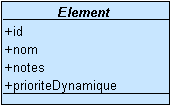
\includegraphics[scale=1]{images/L3/structureDonnee/element.png}
	\caption{La classe Element}
	\label{fig:element}
\end{figure}

\subsubsection{Tache}

	La classe \code{Tache} représente une tâche. Elle possède les attributs suivants:
	\begin{description}
		\item[priorite]: la priorité fixée par l'utilisateur.
		\item[tauxEffort]: le taux d'effort demandé par la tâche.
		\item[liens]: liste des liens internet liés à la tâche.
		\item[tags]: la liste des tags associés à cette tâche.
		\item[isActive]: détermine si la tâche est activée ou non.
	\end{description}

\begin{figure}[htbp]
	\centering
		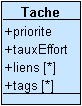
\includegraphics[scale=1]{images/L3/structureDonnee/tache.png}
	\caption{La classe Tache}
	\label{fig:tache}
\end{figure}

\subsubsection{Projet}

Nous avons décidé de spécifier deux types de projets : ordonné ou non.
Un projet ordonné permet de gérer des dépendances entre les tâches qui le composent (par exemple la deuxième tâche dépend de la première d'un même dossier).
Nous avons choisi cette méthode car cela permet d'avoir des dépendances en arborescence, et donc évite les cycles de dépendance qu'il pourrait y avoir si la dépendance n'était qu'un attribut d'une tâche (ou ici d'un élément).
Nous avons donc une classe abstraite Projet, et deux classes concrètes \code{ProjetOrdonne} et \code{ProjetNonOrdonne}.
Chaque classe concrète peut alors choisir la représentation de sa liste interne.

	La classe \code{Projet} représente un ensemble de tâches. Un projet possède les attributs suivants:
	\begin{description}
		\item[listeElement]: les éléments contenus dans  le projet.
	\end{description}

\begin{figure}[htbp]
	\centering
		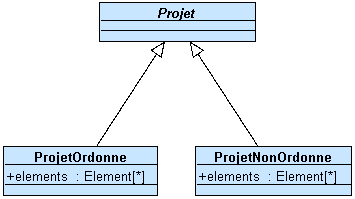
\includegraphics[scale=1]{images/L3/structureDonnee/projets.png}
	\caption{La classe Projet}
	\label{fig:Projet}
\end{figure}

\subsection{Contexte}

	La classe \code{Contexte} représente le contexte associé à une tâche (cf figure \ref{fig:Contexte}). Elle possède les attributs suivants:
	\begin{description}
		\item[nom]: le nom du contexte.
	\end{description}

\begin{figure}[htbp]
	\centering
		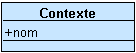
\includegraphics[scale=1]{images/L3/structureDonnee/contexte.png}
	\caption{La classe Contexte}
	\label{fig:Contexte}
\end{figure}

\subsection{Echeancier}

	La classe \code{Echeancier} représente l'échéancier d'une tâche (cf figure \ref{fig:Echeancier}). Elle possède les attributs suivants:
	\begin{description}
		\item[dateDebut]: La date du début de la tâche.
		\item[echeance]: l'écheance de la tâche.
		\item[frequence]: la fréquence de répétition de la tâche.
		\item[dateArret]: la date d'arrêt de la répétition.
	\end{description}

\begin{figure}[htbp]
	\centering
		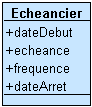
\includegraphics[scale=1]{images/L3/structureDonnee/echeancier.png}
	\caption{La classe Echeancier}
	\label{fig:Echeancier}
\end{figure}

\subsection{Contact}

	La classe \code{Contact} représente les contacts auxquelles les tâches peuvent être associées (cf figure \ref{fig:Contact}). Elle possède les attributs suivants:
	\begin{description}
		\item[nom]: le nom du contact.
		\item[eMail]: son adresse e-mail.
		\item[telephone]: son numéro de téléphone.
		\item[adresse]: son adresse postale.
	\end{description}

\begin{figure}[htbp]
	\centering
		
\includegraphics[scale=1]{images/L3/structureDonnee/contact.png}
	\caption{La classe Contact}
	\label{fig:Contact}
\end{figure}

\subsection{Compte}

La classe \code{Compte} représente le compte auquel est associé un login.
C'est cette classe qui contient l'ensemble des éléments (tâches et projets) d'un utilisateur (cf figure \ref{fig:compte}).
Elle possède les attributs suivants:
	\begin{description}
		\item[nom]: le login du compte.
		\item[mdp]: le mot de passe du compte.
	\end{description}

\begin{figure}[htbp]
	\centering
		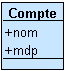
\includegraphics[scale=1]{images/L3/structureDonnee/compte.png}
	\caption{La classe Compte}
	\label{fig:compte}
\end{figure}

\subsection{Ensemble de la structure de donnée}

Voici donc la corrélation des divers éléments de notre structure de donnée (cf figure \ref{fig:structure}).

\begin{figure}[htbp]
	\centering
		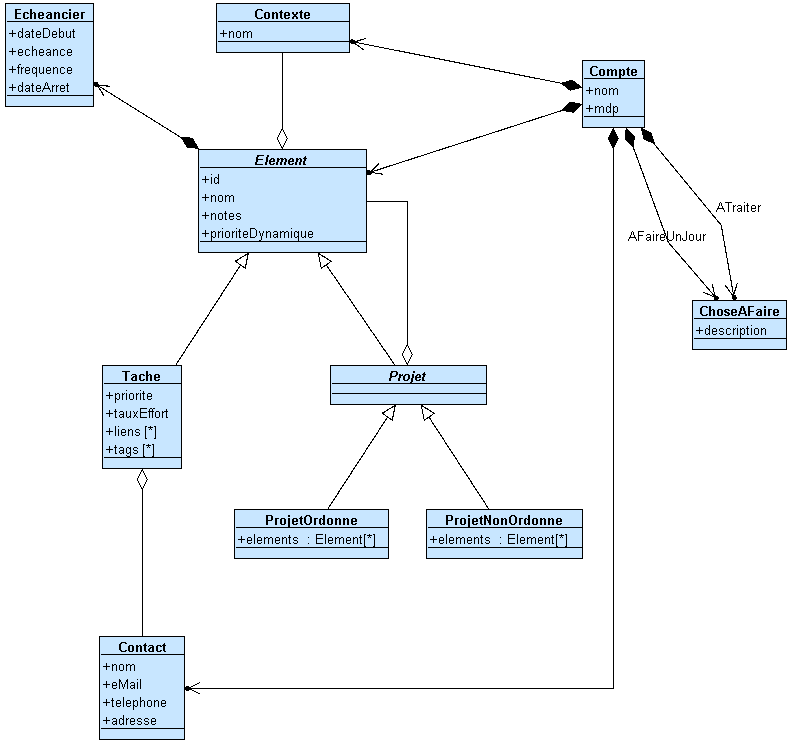
\includegraphics[width=15cm]{images/L3/structureDonnee/comptes.png}
	\caption{La structure de donnée}
	\label{fig:structure}
\end{figure}

\section{Conclusion}

Maintenant que les frontières du système sont établies, nous allons pouvoir détailler chaque composant défini précédemment.


%
% Architecture
%
\chapter{Architecture}

\minitoc


\section*{Introduction}
Maintenant que tous les composants ont été défini, on peut se pencher plus en détails sur les différents niveaux composant notre logiciel et spécifier comment on passe du modèle architectural au modèle physique. Pour faire cela, on va définir sous quelle forme de tables relationnelles nos classes pourront persister, expliquer les patrons de conceptions que nous avons utilisé dans notre modèle de classes et comment on génère le code à partir de celui-ci.


\section{Architecture physique}

%%Intro
	
Le logiciel lourd que nous écrivons se découpe en différentes couches : 

%% Image

\begin{figure}[htbp]

		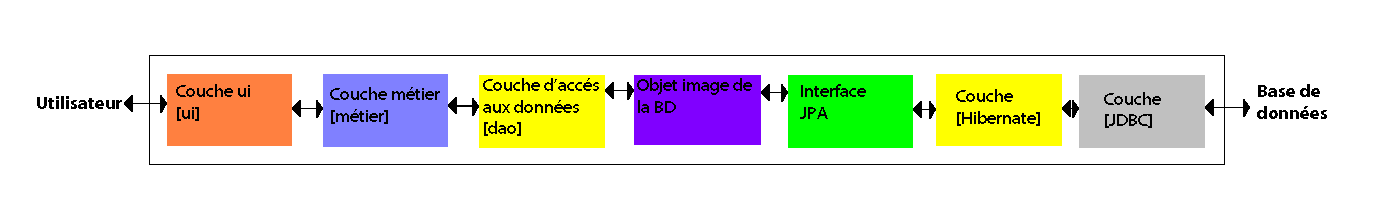
\includegraphics[width=18cm]{images/ArchitecturePhysique.png}
	\caption{Architecture de l'application}
	\label{ArchitectureDeLApplication}
\end{figure}

%% Explication de l'image
%% Ajouter pour chaque couche un exemple de quel code est représenté par cette couche

\begin{enumerate}
\item la couche [ui] (User Interface) est la couche qui dialogue avec l'utilisateur via une interface graphique. Elle a pour rôle de fournir des données provenant de l'utilisateur à la couche [2] ou bien de présenter à l'utilisateur des données fournies par la couche [2].
\begin{itemize}
\item Représente les fenêtres Utilisateur.
\end{itemize}

\item la couche [2], appelée ici [metier] est la couche qui applique les règles dites métier, c.a.d. la logique spécifique de l'application, sans se préoccuper de savoir d'où viennent les données qu'on lui donne, ni où vont les résultats qu'elle produit.
\begin{itemize}
\item Représente les différentes fonctions de notre programme : collecter traiter ...
\end{itemize}

\item la couche [3], appelée ici [dao] (Data Access Object) est la couche qui fournit à la couche [2] des données pré-enregistrées (fichiers, bases de données, ...) et qui enregistre certains des résultats fournis par la couche [2].
\begin{itemize}
\item La couche dao rassemble les descripteurs des classes qui seront "persistées".
\end{itemize}

\item La couche [4] des objets-images de la BD est appelée "contexte de persistance". Elle fait le lien entre la couche [dao] qui s'appuie sur Hibernate pour faire des actions de persistance (CRUD, create - read - update - delete).  Cette couche, fournie par la couche inférieure [5] représente la base de donnée : on n'utilise pas directement la base de données physique.
\begin{itemize}
\item Appellée lors des ajouts suppressions ... sur la base de données.
\end{itemize}

\item L'interface [JPA] est un ensemble générique d'interfaces permettant des accès plus bas niveau (sur les couches physiques comme la base de données) sans avoir à mettre les mains dans le camboui. Elle permet de rendre toutes ses couches inférieures réutilisables.
\begin{itemize}
\item Chaque classe qui doit être "persistée" doit posséder un classe Entity faisant justement partie de la couche JPA.
\end{itemize}

\item La couche [Hibernate] traduit les actions de persistence en ordres SQL.Pour les actions d'interrogation de la base (le SQL Select), Hibernate fournit au développeur, un langage HQL (Hibernate Query Language) pour interroger le contexte de persistance [4] et non la BD elle-même. Cette couche fait le pont entre le monde relationnel et le monde objet.
\begin{itemize}
\item Hibernate est une couche transparente et fourni des outils, et donc n'apparait pas directement dans le code.
\end{itemize}

\item la couche [JDBC] est la couche standard utilisée en Java pour accéder à des bases de données. C'est ce qu'on appelle habituellement le pilote Jdbc du SGBD.
\begin{itemize}
\item Représente la base de données physique.
\end{itemize}

\end{enumerate}

\paragraph*{}
Nous obtenons ainsi une chaîne reliant l'utilisateur (hors logiciel) jusqu'à la base de données (couche la plus physique) contenant ses informations. Chaque couche possède des règles et discute avec les couches l'entourant. Chaque couche modifie ou interprète les informations pour la couche inférieure/supérieure et permet ainsi le fonctionnement du logiciel.


\section{Schémas des bases de données}
	
	\subsection{Logins et mots de passe}

	La base de données des identifiants n'est jamais chargé. Quand un utilisateur entre un mot de passe, le programme chiffre celui-ci et parcourt le fichier pour comparer si le mot de passe chiffré qu'il vient de générer et celui stocké pour cet utilisateur sont les mêmes. Cette opération est simple et ne doit être faite que peu souvent, c'est pourquoi on peut se permettre de ne pas charger le contenu du fichier dans une base de données.

	\subsection{Java Persistence API}
	
	Les comptes sont stockés localement dans des fichiers et lorsque l'utilisateur a entré un mot de passe correct, le programme charge le compte lié à ce mot de passe dans la base de donnée pour y accéder et modifier les informations. C'est ainsi que la persistance est géré pour les comptes hors connexion ou dont la connexion est inactive.
	\paragraph*{}
	Le compte est géré de manière différente selon le programme (classes) et la base de données (tables). On doit donc écrire des schémas de "traduction" de la base de données relationnelle aux classes. Nous avons choisi de créer une table par chemin d'héritage.
	\paragraph*{}
	On commence en réalisant les schémas de toutes les classes isolées (ne dépendant pas de chemins d'héritage) :\\

	\begin{figure}[htbp]

		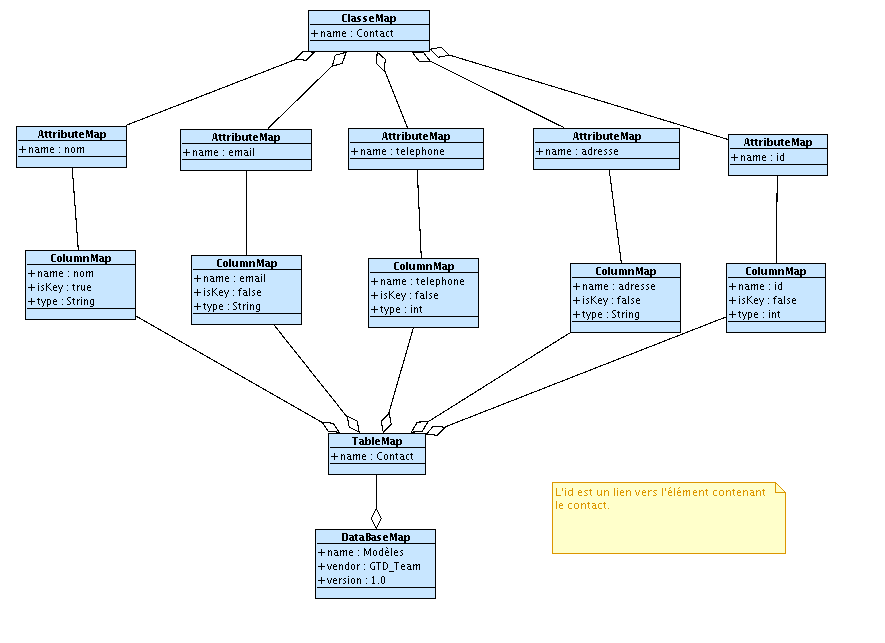
\includegraphics[width=18cm]{images/L4/ContactDBS.png}
	\caption{Schéma de la base de données : Table Contacts}
	\label{ContactDBS}
\end{figure}
La table "Contact" \ref{ContactDBS} contient les colonnes liées aux attributs de la classe associée, plus l'id de la tâche, du projet ou directement du compte auquel elle est liée. \\


\begin{figure}[htbp]

		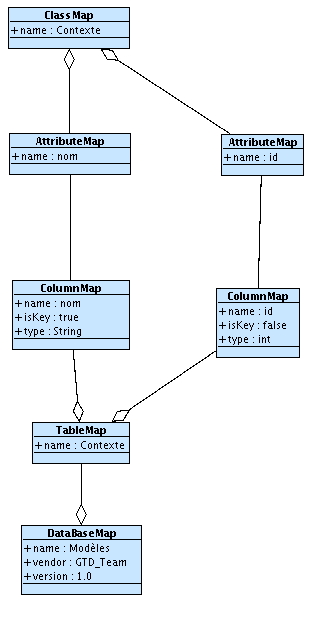
\includegraphics[width=10cm]{images/L4/ContexteDBS.png}
	\caption{Schéma de la base de données : Table Contexte}
	\label{ContexteDBS}
\end{figure}
De même que la classe précédente, la table "Contexte" \ref{ContexteDBS} contient l'id de l'élément qui l'utilise (de même pour les tables Tags \ref{TagDBS}, "Echeancier" \ref{EcheancierDBS} et "Participant" \ref{ParticipantDBS} ).\\

\begin{figure}[htbp]

		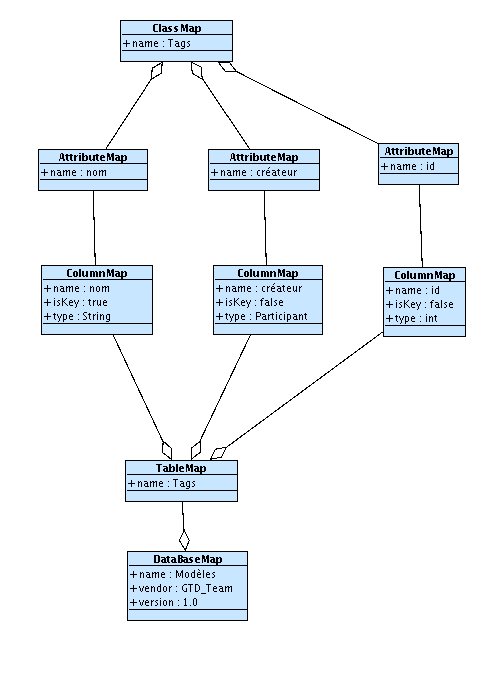
\includegraphics[width=14cm]{images/L4/TagsDBS.png}
	\caption{Schéma de la base de données : Table Tags}
	\label{TagDBS}
\end{figure}


\begin{figure}[htbp]

		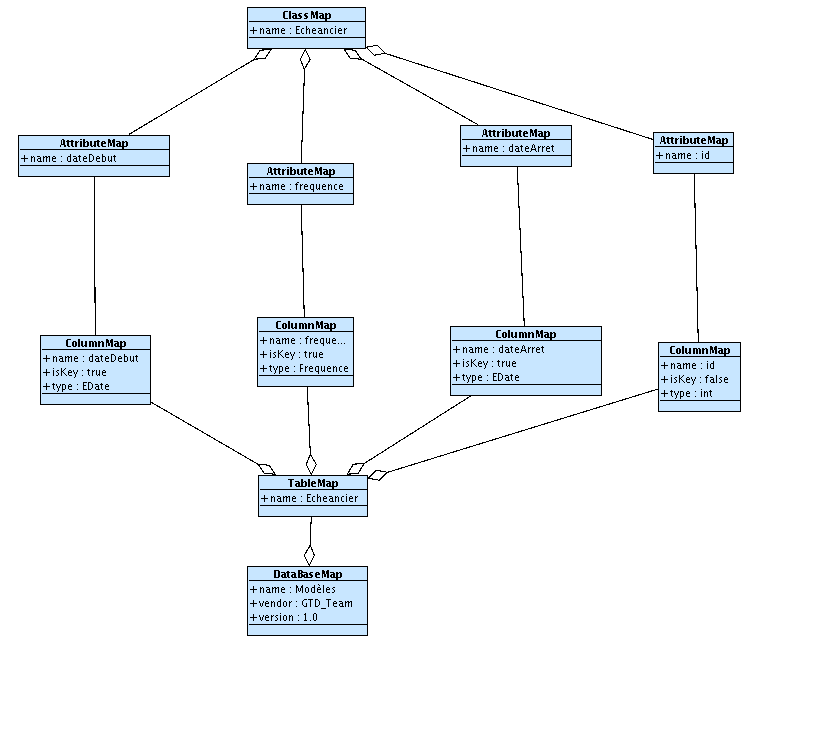
\includegraphics[width=18cm]{images/L4/EcheancierDBS.png}
	\caption{Schéma de la base de données : Table Echeancier}
	\label{EcheancierDBS}
\end{figure}


\begin{figure}[htbp]

		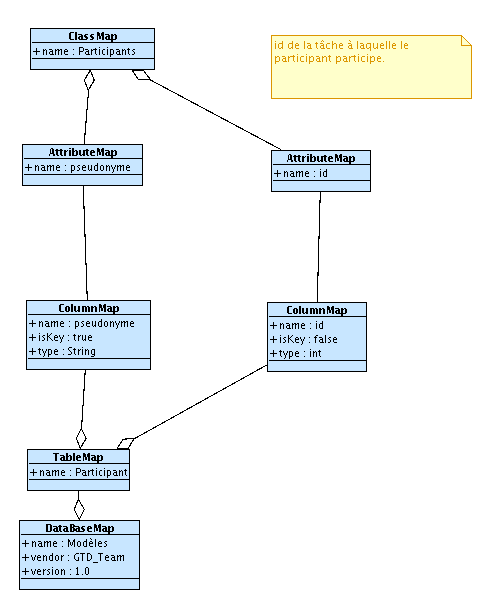
\includegraphics[width=16cm]{images/L4/ParticipantDBS.png}
	\caption{Schéma de la base de données : Table Participant}
	\label{ParticipantDBS}
\end{figure}



\begin{figure}[htbp]

		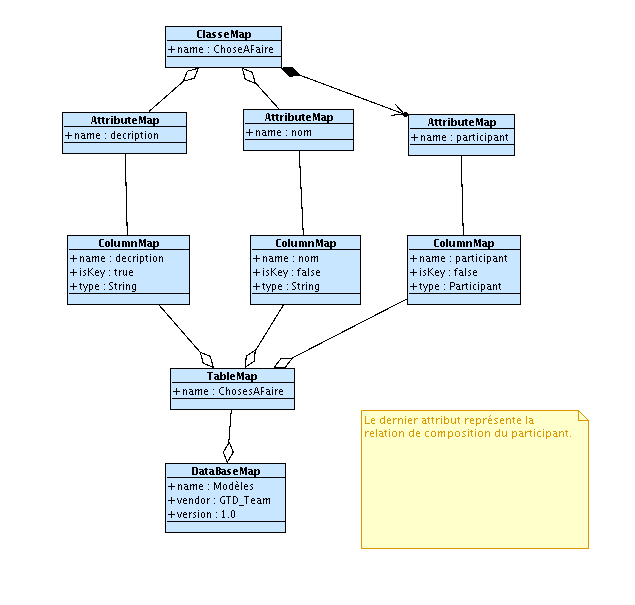
\includegraphics[width=18cm]{images/L4/ChoseDBS.png}
	\caption{Schéma de la base de données : Table Chose à faire}
	\label{ChoseDBS}
\end{figure}
A la différence des tables précédentes, la table "ChoseAFaire" \ref{ChoseDBS} contient une colonne pour mémoriser le participant de l'action (il peut ne pas y en avoir).\\

\paragraph*{}
Puis on termine par les classes héritant d'attributs communs provenant de la classe "Élément" :\\

\begin{figure}[htbp]

		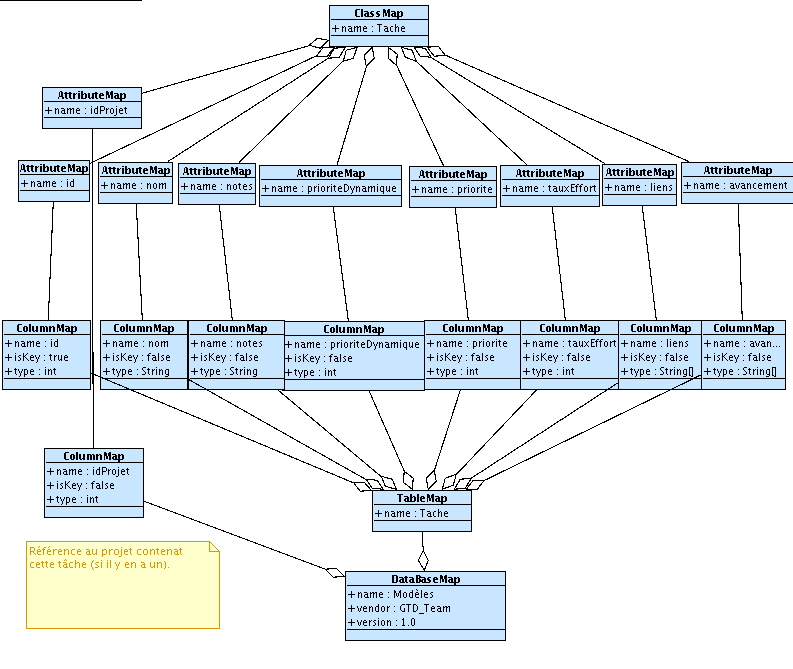
\includegraphics[width=18cm]{images/L4/TacheDBS.png}
	\caption{Schéma de la base de données : Table Tâches}
	\label{TacheDBS}
\end{figure}
\paragraph*{}
On retrouve donc dans la table "Tâche" \ref{TacheDBS} tous les attributs de la classe "Élément" et ceux de la classe "Tâche", plus un attribut référençant le projet contenant cette tâche (s'il y en a un).\\


\begin{figure}[htbp]

		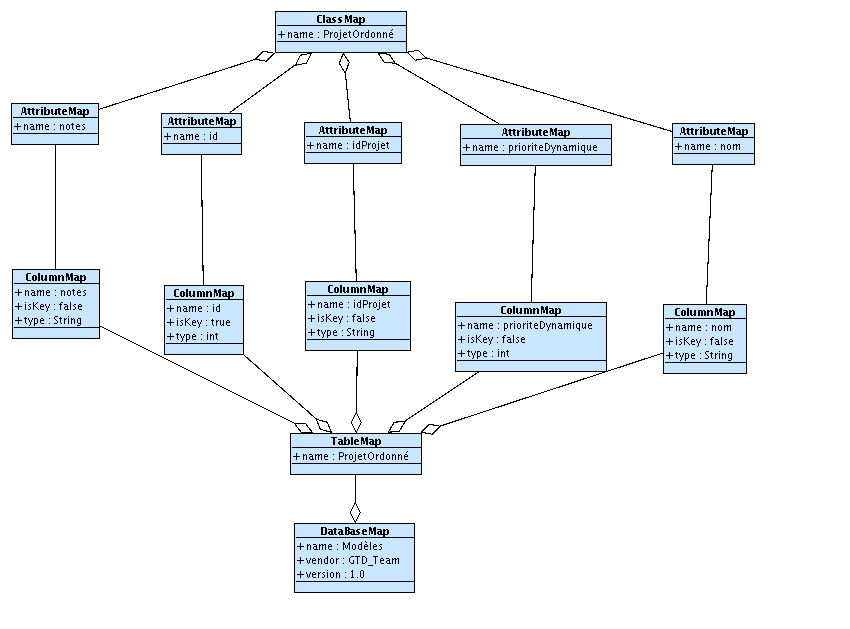
\includegraphics[width=18cm]{images/L4/ProjetNonOrdDBS.png}
	\caption{Schéma de la base de données : Table Projets Non Ordonnés}
	\label{ProjetNonOrdDBS}
\end{figure}
\paragraph*{}
De même pour un "Projet Non Ordonné" \ref{ProjetNonOrdDBS} qui peut être le sous-projet d'un autre projet.\\


\begin{figure}[htbp]

		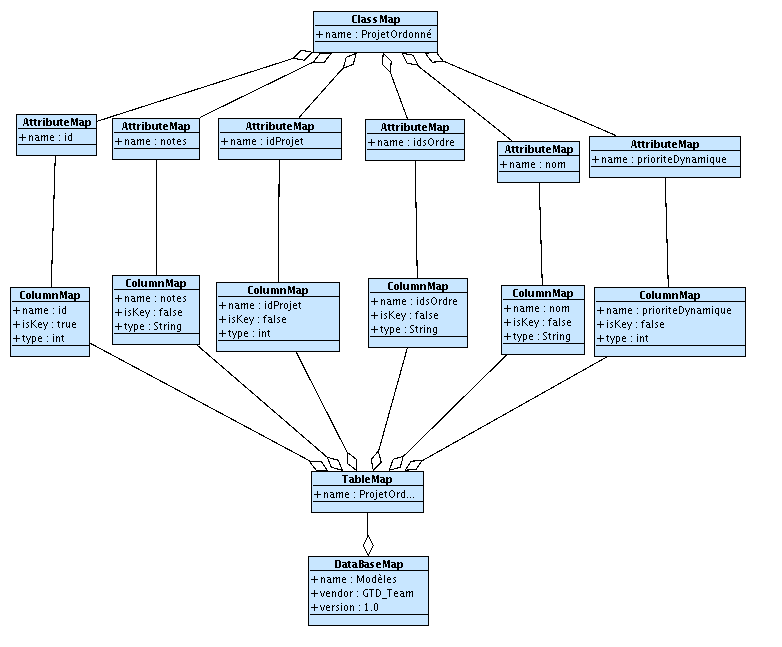
\includegraphics[width=18cm]{images/L4/ProjetOrdDBS.png}
	\caption{Schéma de la base de données : Table Projets Ordonnés}
	\label{ProjetOrdDBS}
\end{figure}
\paragraph*{}
Les "Projets Ordonnés" \ref{ProjetOrdDBS} peuvent aussi être des sous-projets mais doivent se "souvenir" de l'ordre des tâches qu'il contienne d'où la chaîne de caractères contenant les ids ordonnés des tâches d'un "Projet Ordonné".


\section{Stéréotypes et étiquettes}
Pour pouvoir implémenter proprement notre logiciel, nous avons utilisé différents patrons de conception pour créer son architecture.


	\subsection{Modèle-Vue-Contrôleur}
	Dans un premier temps, nous avons découper nos classes en 3 parties. Ce qui nous a permis d'y voir un peu plus clair dans ce que fait chaque composants logiciels. Dans notre diagramme de classes, la partie Vue n'apparaît pas car elle est plus extérieure; mais elle est bien présente dans notre logiciel. 
	
	\subsection{Projets : patron Composite}
	Selon notre diagramme de classes, un Projet est un Élément. Seulement nous avons défini depuis le début qu'un Projet peut contenir des sous-Projets; c'est pourquoi nous avons utilisé ici le patron Composite.
	
	\subsection{Méthode GTD : patron Stratégie}
	La partie Organisation de la méthode GTD est une partie complexe et nous avons choisi d'utiliser le patron Stratégie pour pouvoir changer facilement son code. Ce qui nous donne la possibilité de changer cette méthode à tout moment pour l'améliorer ou changer complètement son code métier.
	
	\subsection{Comptes : patron Visiteur}
	On utilise le patron Visiteur pour pouvoir accéder facilement au différentes valeurs stockées dans le Modèle.
	


\section{Règles de traduction}

On utilise les règles suivantes de traduction de l'UML vers Java avec Acceleo:
\begin{itemize}
\item Chaque package  dans le diagramme de classe se transforme en \textit{Package Java};
\item Chaque classe génère une \textit{Class Java} ainsi que son constructeur;
\item Chaque interface génère des \textit{Interfaces Java};
\item Une propriété donne une méthode;
\item Un attribut est privé et on génère des \textit{Getters/Setters};
\item Pour les attributs avec une multiplicité supérieur, on place l'attribut Java dans une \textit{LinkedList} et on ajoute des méthodes d'ajout et de suppression dans cette liste;
\item Si une classe hérite d'une autre, on rajoute le \textit{extend};
\item Une classe qui implémente une interface se voit ajouter \textit{implements}et on génère les méthodes de l'interface que la classe implémente.
\end{itemize}

\paragraph*{}
Ces quelques règles nous permettent de générer du code sur lequel nous pourrons "greffer" le code métier de notre application.

\section*{Conclusion}
Puisque nous avons défini l'architecture globale de notre logiciel, nous pouvons dès à présent nous intéresser aux détails des composants et ainsi définir tous les détails précédant la partie de codage visant à remplir le code généré.


	
	
	
	

\chapter{Conception détaillée}

\section*{Introduction}
Le dernier pas dans la conception de notre logiciel est de spécifier en détails tous les composants et leur rôles. Nous aurons de ce fait décrit tous les aspects de notre programme et pourrons le développer sans ambiguïtés.

\section{Répertoire de décisions}

Mais avant de rentrer dans les détails de la conception, nous devons préciser les modifications apporter au modèle durant le développement.\\
Pour rappel, le modèle après analyse était la figure \ref{ddcanalyse}.

\begin{figure}[!ht]
\begin{center}
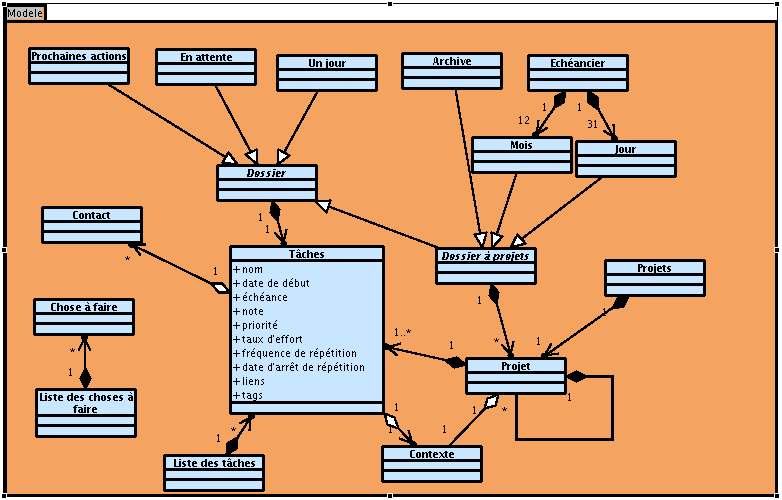
\includegraphics[width=12cm]{images/DiagrammedeClasse.png}
\caption{Diagramme de classes du modèle après analyse}
\label{ddcanalyse}
\end{center}
\end{figure}

Et maintenant, le diagramme de classe est représenté par la figure \ref{ddcfinal}.

\begin{figure}[!ht]
\begin{center}
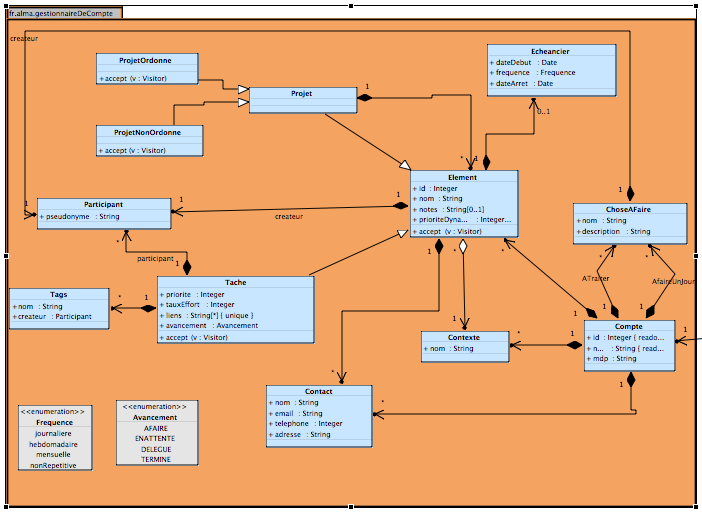
\includegraphics[width=12cm]{images/ClassDiagram.png}
\caption{Diagramme de classes du modèle à la fin du projet}
\label{ddcfinal}
\end{center}
\end{figure}


Les modifications sont nombreuses :
\begin{itemize}
\item Suppression de la classe Mois (Les échéances sont stockées dans l'échéancier et les tâches ou projets qui l'utilisent pointent dessus);
\item Suppression de la classe Jour (comme Mois);
\item Suppression de Archive (les éléments contiennent un état pour renseigner si ils sont actifs ou non);
\item Suppression des "dossiers" Dossier/Dossier à projets/Projets (la version informatique rend obsolète l'utilisation de dossiers);
\item Suppression de Prochaines Actions (élément visuel, les tâches sont afficher en fonction des choix de l'utilisateur);
\item Suppression de Liste des Tâches (affichage des tâches, pas besoin de les stocker ensemble);
\item Modification de Liste des Choses à faire (attribut d'une autre classe);
\item Modification de Contacts et Tags (ajout d'attributs);
\item Modification de En Attente (contenu dans l'état de l'élément);
\item Modification de Un Jour (attribut d'une autre classe);
\item Ajout de Participants (nécessaire pour les éléments ordonnés et connaître les dépendances);
\item Ajout de Projet Ordonné et de Projet Non Ordonné (sous classes de Projet);
\item Ajout de Éléments (pour regrouper les attributs commun de Tâche et Projet, et implémenter le patron Composition)
\item Ajout de Compte (contient toutes les autres classes).
\end{itemize}

Ainsi nous obtenons le diagramme de classe de la figure \ref{ddcfinal} et pouvons ainsi commencer la conception détaillée.

\section{Diagrammes statiques et dynamiques}

Le diagramme de classe du modèle n'est pas le seul à avoir changé, le reste du diagramme de classe a lui aussi eu des modifications(Voir figure \ref{ddctotal}).

\begin{figure}[!ht]
\begin{center}
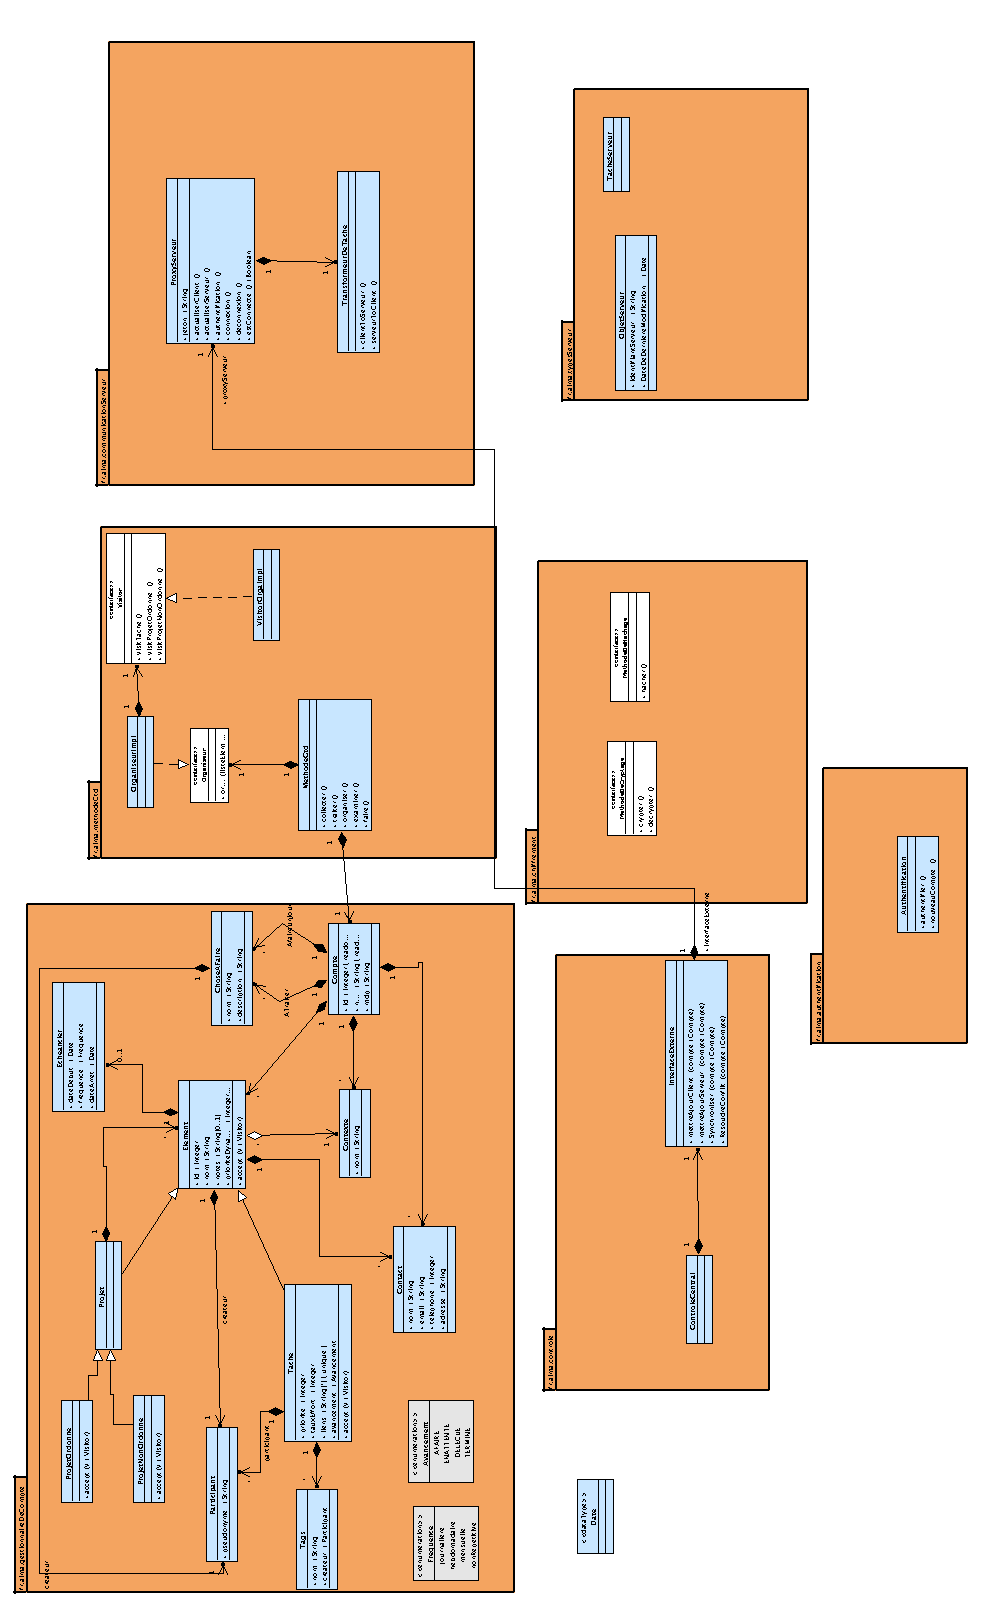
\includegraphics[width=14cm]{images/FullClassDiagram.png}
\caption{Diagramme de classes final}
\label{ddctotal}
\end{center}
\end{figure}

On peut voir les différentes interactions entre les composants décrits dans le chapitre "Spécification des Composants".


\section{Spécification des classes}

Cette section comporte une liste de toutes les classes en spécifiant pour chacune d'elles ses invariants.\\


\subsection*{Package : Gestionnaire de Compte}

\subsubsection*{Classe : Compte} 
\begin{itemize}
\item Nom jamais vide
\item Mot de passe jamais vide
\end{itemize}


\subsubsection*{Classe : Chose A Faire}
\begin{itemize}
\item Nom jamais vide
\item description jamais vide
\end{itemize} 

\subsubsection*{Classe : Contexte}
\begin{itemize}
\item Nom jamais vide
\end{itemize} 

\subsubsection*{Classe : Contact}
\begin{itemize}
\item Le couple nom/adresse unique
\item Nom jamais vide
\item Adresse jamais vide
\end{itemize} 

\subsubsection*{Classe : Élément}
\begin{itemize}
\item Nom jamais vide
\end{itemize} 

\subsubsection*{Classe : Participant}
\begin{itemize}
\item Id unique
\item Pseudonyme jamais vide
\end{itemize} 

\subsubsection*{Classe : Échéancier}
\begin{itemize}
\item Triplet d'attributs unique
\end{itemize}

\subsubsection*{Classe : Tag}
\begin{itemize}
\item Nom non vide
\item Nom unique
\end{itemize}

\section*{Conclusion}
Toutes les étapes de l'analyse étant terminées, nous pouvons finalement commencé l'implémentation qui est facilitée grâce à l'analyse poussée que nous avons réalisé. La génération de code à partir de notre modèle nous fera gagner du temps et l'utilisation de frameworks, tels Hibernate, nous facilitera la tâche.

\chapter*{Conclusion}

Le développement de cette application nous a permis d'aborder de nouvelles méthodes telles que la génération de code, et d'approfondir des méthodes vu dans d'autres modules telles que la gestion de la persistance, les EJB.. Nous avons ainsi pu utiliser pleinement de nouveaux frameworks et de nouvelles méthodes de travail.
Nous avons aussi pu mieux maîtriser la gestion et la répartition du travail au sein de notre groupe en même temps que de travailler sur un projet de gestion du travail à faire.
L'interaction entre les modules s'est révélée aisé grâce aux professeurs qui nous ont guider.
Ce projet nous a par ailleurs détailler niveau par niveau les différents pas pour donner vie à une idée (passage de l'idée jusqu'au produit final).


\begin{thebibliography}{99}

\bibitem{wikipedia}
Wikipedia, Getting Things Done : \\
\url{http://en.wikipedia.org/wiki/Getting_Things_Done}

\bibitem{gettingThingsGnome}
Getting Things GNOME ! : \\
\url{http://gtg.fritalk.com/}

\end{thebibliography}


\end{document}

